% === Cours de Java
% === Fichier principal
\usetheme[secheader]{Madrid}
\usepackage{java}

\title{Le Langage Java}
\subtitle{1\iere\ ann\'ee}
\institute[HEB-�SI]{Haute �cole de Bruxelles --- �cole Sup�rieure d'Informatique}    
\date[2014 --- 2015]{Ann�e acad�mique 2014 / 2015}
\author[]{ \small
  J.~Beleho (bej) \and 
  C.~Leruste (clr) \and
  M.~Codutti (mcd) \and
  P.~Bettens (pbt) \and
  F.~Servais (srv) \and
  C.~Leignel (clg) \and
  D.~Nabet (dna) \and
  J.~Lechien (jlc)
}

\begin{document}

% ===== Page de titre ======
\begin{frame}
\titlepage
\end{frame}

% ===== Table des mati�res ======

\setbeamertemplate{section in toc}[square] 
\setbeamerfont{section in toc}{size=\small}

\begin{frame}{Liste des s�ances }
	\vspace{-40pt}
	\tableofcontents[hideallsubsections,sections={1}]
	\vspace{-40pt}
	\tableofcontents[hideallsubsections,sections={2}]
	\vspace{-40pt}
	\tableofcontents[hideallsubsections,sections={3}]
	\vspace{-40pt}
	\tableofcontents[hideallsubsections,sections={4}]
	\vspace{-40pt}
	\tableofcontents[hideallsubsections,sections={5}]
	\vspace{-40pt}
	\tableofcontents[hideallsubsections,sections={6}]
	\vspace{-40pt}
	\tableofcontents[hideallsubsections,sections={7}]
	\vspace{-40pt}
	\tableofcontents[hideallsubsections,sections={8}]
	\vspace{-40pt}
	\tableofcontents[hideallsubsections,sections={9}]
	\vspace{-40pt}
	\tableofcontents[hideallsubsections,sections={10}]
	\vspace{-40pt}
	\tableofcontents[hideallsubsections,sections={11}]
	\vspace{-40pt}
	\tableofcontents[hideallsubsections,sections={12}]
\end{frame}


% ===== Les diff�rentess s�ances =====
% == S�ance 1
\section{Objectifs, �valuations et introduction}
\leconwithtocquote{\og\ I really hate this darn machine;
I wish that they would sell it.
\\It won't do what I want it to,
but only what I tell it. \fg
\\Anonyme}

\subsection{Objectifs}

\imgfullw{../img/goal_by_zi3000.jpg}
	{Notre objectif $\cdots$ \hfill $\cdots$ votre objectif}
	{http://zi3000.deviantart.com/art/goal-59036635}

\begin{frame}{Objectifs du cours}
\begin{itemize}
	\item initiation � la programmation 
	\item apprentissage de bons comportements
	\item impl�mentation sur un OS (\textit{operating system})
\end{itemize}
\end{frame}

\begin{frame}{Liens avec les autres cours}
	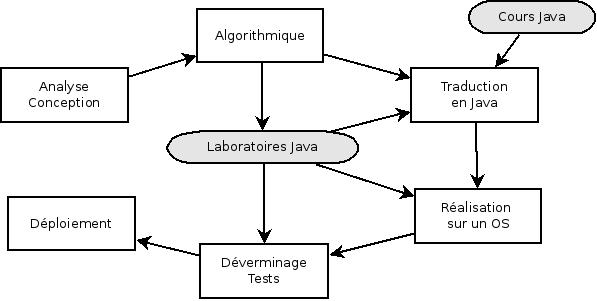
\includegraphics[width=\linewidth]{../img/etapes-SI.jpeg}
\end{frame}


\subsection{Moyens}

\begin{frame}{Supports et ressources}
\emph{Rien} 
\begin{itemize}
  \item pas de syllabus;
  \item pas de livre;
\end{itemize}
\bigskip
\emph{Quoique}
\begin{itemize}
	\item les slides sur \href{https://github.com/HEB-ESI/DEV1-JAV-Slides}{github};
	\item des liens, des documents, $\cdots$ sur \href{https://elearning.esihheb.be}{po�SI}
	\item un forum de discussion, (\href{http://fora.namok.be}{fora})
\end{itemize}
\end{frame}

\subsection{�valuations}

\imgfullw{../img/OMG_Spaghetti_O__s_by_billyunderscorebwa.jpg}
	{\centering\huge\color{white}{�valuation � quelle sauce ?}}
	{http://framedbynature.deviantart.com/art/OMG-Spaghetti-O-s-81044629}

\begin{frame}{�valuation}
	�valuation de l'unit� d'enseignement (UE), 
	\\une cote pour toutes les activit�s d'apprentissage (AA):
	\bigskip
	\begin{center}
		{\color{darkgray}\large\bf 
			$\overbrace{\text{ALG - JAV - LAJ}}^{\text{DEV1}}$
		}
	\end{center}
\end{frame}


% === Cours de Java
% === Chapitre : Introduction

\subsection{Concepts}

\imgfullw{../img/coffeemug.jpg}{
	\Large\textbf{\color{white}programmer}\\
	\textit{\color{gray}[proh-gram-er]}\\
	{\large\color{white}an organism that turn caffeine into software}
}{https://www.flickr.com/photos/secret_canadian/22234285/sizes/o/}

\begin{frame}{D�finitions}
D�finissons les concepts suivants :
\begin{itemize}
\item Un \emph{programme} ?
\item \emph{Programmer} ?
\item Un \emph{langage de programmation} ? 
\item Diff�rence entre \emph{langue} et \textit{langage} ?
\end{itemize}
\end{frame}


\begin{frame}{Un programme}
La seule chose dont est capable un ordinateur est de r�aliser extr�mement rapidement des instructions �l�mentaires
\par\bigskip
Toute t�che qu'on veut lui confier doit donc �tre pr�alablement d�crite comme une suite s�quentielle d'instructions (un programme)
\note[item]{\url{http://en.wikipedia.org/wiki/Source_lines_of_code} donne des exemples de taille de programmes}
\end{frame}



\begin{frame}{Un langage}
\emph{Une classe de langages est adapt�e � une classe de probl�mes \dots\ et ces probl�mes �voluent dans le temps \dots}
\note[item]{On peut aborder ici l'historique des langages : machine, assembleur, haut niveau, structur�, orient� objet, fonctionnels, orient�s aspects\dots}
\end{frame}


\subsection{Traduction}

\begin{frame}{Le probl�me de la traduction}
Un ordinateur ne comprend que le langage machine. N�cessit� d'une \emph{traduction}
\bigskip
\begin{center}
\begin{tabular}{c|c}
\emph{Compilation} & \emph{Interpr�tation} \\ \hline
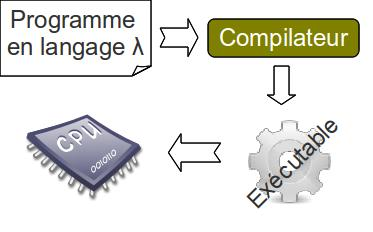
\includegraphics[scale=.35]{../img/java-jvm-compil} &
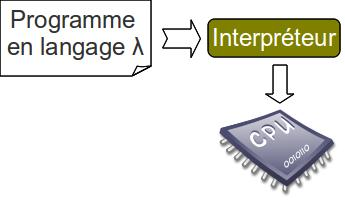
\includegraphics[scale=.35]{../img/java-jvm-interp} \\
\textit{\small traduit d'une traite} & \textit{\small traduit morceau par morceau} \\
\textit{\small avant l'ex�cution} & \textit{\small au moment de l'ex�cution} \\
\end{tabular} 
\end{center}
\note[item]{Faire une comparaison des avantages/inconv�nients}
\end{frame}

\full[bluepigment]{
	\begin{center}
		\color{white}
		{\huge\bf Et \sigle{Java} ?}
		\bigskip\\
		{\large Compil� ou interpr�t� ?}
	\end{center}
}



% == Cours de Java
% === Chapitre : Introduction

\begin{frame}{La machine virtuelle}
	\sigle{Java} a une approche mixte la \emph{machine virtuelle \sigle{Java}} (\sigle{JVM})  
\medskip
\begin{center}
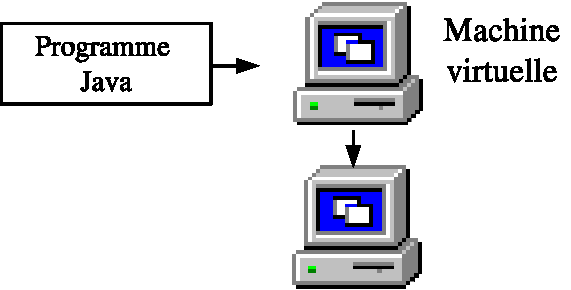
\includegraphics[scale=.8]{../img/java-jvm-jvm1} 
\end{center} 
\end{frame}

\full[bluepigment]{
	\begin{center}
		\Large\bf\color{azuremist}
		D'abord compil� \par ensuite interpr�t�
	\end{center}
}

\begin{frame}{La machine virtuelle}
\begin{center}
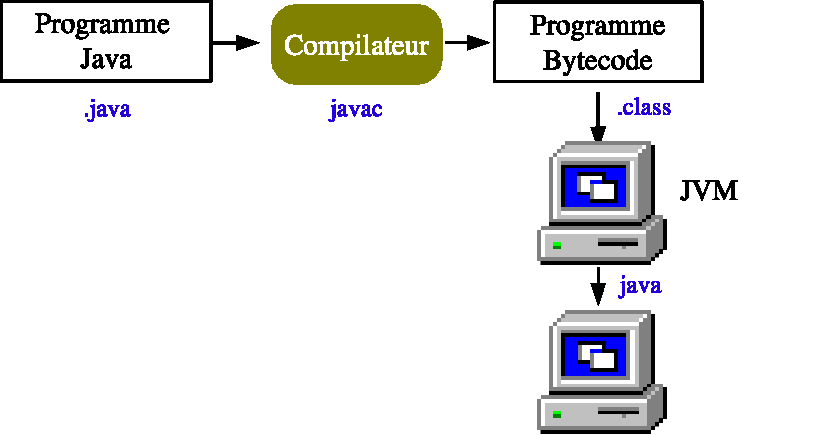
\includegraphics[scale=0.8]{../img/java-jvm-jvm2} 
\end{center}
\end{frame}

\imgfullw{../img/true-evolution.jpg}
	{\color{white}\textit{timeline \sigle{Java}}}
	{http://www.tshirthell.com/funny-shirts/true-evolution}

\begin{frame}[fragile]{Historique de \sigle{Java}}
\begin{itemize}
\item [\emph{92}] \sigle{SUN} cr�e \sigle{oak} (syst�mes embarqu�s).
\\Auteur: James Gosling
\item [\emph{94}] Adapt� � Internet gr�ce aux \emph{applets}. 
\\Devient \sigle{Java}
\item [\emph{96}] Premi�re version stable et gratuite de \sigle{JDK} 
\item [\emph{98}] Sortie de \sigle{Java 2}
\item [\emph{05}] Version \verb|1.5| de \sigle{Java 2}
\item [\emph{09}] \sigle{Oracle} rach�te \sigle{Sun} (et donc \sigle{Java})
\item [\emph{11}] Version \verb|1.7| (Java 7, en GPL)
\item [\emph{14}] Version \verb|1.8| (Java 8)
\end{itemize}
\end{frame}

\begin{frame}
	
\includegraphics[scale=.5]{../img/icon_39938.png}
	\begin{itemize}
		\item \sigle{Java} est-il install� sur ma machine ? 
		\item Puis-je commencer � �crire un programme \sigle{Java} ? 
		\item Qu'ai-je pris comme note ? 
	\end{itemize}
	\note[item]{Introduire les termes : JRE, JDK, ME, SE, EE}
	\note[item]{En fait, il y a un slide l�-dessus dans la s�ance 2}
\end{frame}


% ==S�ance 2
\section{D�velopper en \sigle{Java}, premier survol}
\leconwithtocquote
{\og There are two ways to write error-free programs;\\only the third one works.\fg \ Alan J. Perlis}

% === Cours de Java
% === Chapitre : Introduction

\subsection{La machine virtuelle}

\begin{frame}
	\begin{center}
		Java est \emph{compil�} puis \emph{interpr�t�}.
	\par
	L'interpr�teur Java est la machine virtuelle (\sigle{JVM})
	\par
	Le langage de bas niveau interpr�t� par la \sigle{JVM} est le \emph{\sigle{bytecode}}
\end{center}
\end{frame}

\begin{frame}{La machine virtuelle}
\begin{center}
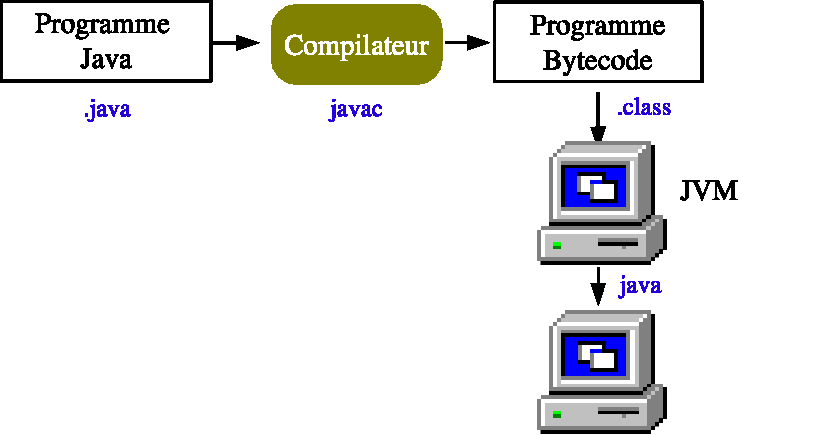
\includegraphics[scale=0.8]{../img/java-jvm-jvm2} 
\end{center}
\end{frame}

\imgfullh{../img/Sun_and_rain_by_emolawn.jpg}
{\begin{flushright}\large\bf\color{ghostwhite} Avantages et\\inconv�nients\end{flushright}}
	{http://emolawn.deviantart.com/art/Sun-and-rain-85676638}


\begin{frame}[fragile]{Exemple: premier programme}
Prenons un exemple \textit{(fichier \code{Hello.java})}
\begin{Java}
// Mon premier programme
public class Hello {
  public static void main(String[] args) {
    System.out.println("Bonjour !");
  }
}
\end{Java}
Compilons-le \texttt{\$ javac Hello.java}
\par
On obtient la version compil�e, le \sigle{bytecode} (\code|Hello.class|)
\par
On peut l'ex�cuter \texttt{\$ java Hello}\\
\texttt{Bonjour !}
\end{frame}

\subsection{Les outils de d�veloppement}

\imgfullh{../img/righttool-3348965007_b3049c78fe_b.jpg}
{\vspace{-1cm}\color{cadetgrey}\Large\bf Fourbir ses armes}
{https://www.flickr.com/photos/ebarney/3348965007/in/photostream/}


\begin{frame}{Les outils de d�veloppement}
Les �ditions de \sigle{Java}
\begin{itemize}
	\item \emph{Java SE} (�dition standard)
	\item \emph{Java ME} (�dition mobile - plus l�ger) 
	\item \emph{Java EE} (�dition entreprise - plus complet)
\end{itemize}
\begin{wrapfigure}{r}{17mm}
	
\includegraphics[width=17mm]{../img/java-download.png}
\end{wrapfigure}
\bigskip
O� trouver \code|javac| et \code|java| ?
\par
\emph{\sigle{JRE}} (\textit{Java Runtime Environment}) \\
\emph{\sigle{JDK}} (\textit{Java Development Kit})
\end{frame}


\full[bluepigment]{\centering\Large\bf\color{azuremist}
	\par\noindent �diter
	\par\noindent Compiler
	\par\noindent Ex�cuter
}

\begin{frame}{Les outils de d�veloppement}
 \par{\bf\Huge 1} 
\begin{itemize}
\item Un \emph{�diteur avec coloration syntaxique}:
	\emph{\sigle{gVim}}, \emph{\sigle{Notepad++}}, \emph{\sigle{nano}}, \dots
\item Gestion manuelle des noms et emplacements des fichiers
\item Compilation et ex�cution en ligne de commande
\end{itemize}
\end{frame}

\begin{frame}{Les outils de d�veloppement}
 \par{\bf\Huge 2}
 \begin{itemize}
	\item Un \textit{\emph{E}nvironnement de \emph{D}�veloppement \emph{I}nt�gr�} : 
	\emph{\sigle{Netbeans}}, \emph{\sigle{Eclipse}}, \dots
  	\item Int�gre tout le processus de d�veloppement  
  \end{itemize}
\end{frame}



% === Cours de Java
% === Chapitre : Survol 

%\subsection{Algorithmes s�quentiels (survol)}
\subsection{Structure g�n�rale d'un programme}

\imgfullw{../img/Life_in_a_frame_by_michaelpaleodimos.jpg}
{}
{http://michaelpaleodimos.deviantart.com/art/Life-in-a-frame-39596992}

\begin{frame}[fragile]{Structure g�n�rale du programme}
	\texttt{\small\$cat NomClasse.java}
\begin{Java}
  public class NomClasse {
    // insert code here
  }
\end{Java}
\bigskip
\bigskip
\emph{Attention} \sigle{Java} est sensible � la casse 
\end{frame}

\begin{frame}[fragile]{La m�thode principale}
	\texttt{\small\$cat NomClasse.java}
\begin{Java}
  public class NomClasse {
    public static void main(String[] args) {
      // insert code here     
    }
  }
\end{Java}
\emph{Exemple}
\begin{Java}
  public class NomClasse {
    public static void main(String[] args) {
      System.out.println("Bonjour !");     
    }
  }
\end{Java}
\end{frame}


\subsection{Commentaires}

\begin{frame}[fragile]{Le commentaire}
Plusieurs mani�res d'ajouter un commentaire 
  \begin{Java}
  // Commentaire sur une ligne
  /* Commentaire sur
     plusieurs lignes */
  \end{Java}
\end{frame}

\subsection{Exemples}

\begin{frame}[fragile]{La m�thode principale}
\emph{Exemples}
\begin{Java}
  public class Exercice1 {
    public static void main(String[] args) {
      System.out.println(3 + 4);     // Affiche la valeur 7
    }
  }
\end{Java}

\begin{Java}
  public class Exercice2 {
    public static void main(String[] args) {
      System.out.println("3 + 4");	// Affiche la chaine 3 + 4
    }
  }
\end{Java}
\end{frame}

\begin{frame}[fragile]{Math.random()}
\begin{Java}
  public class Exercice3 {
    public static void main(String[] args) {
    	  // Affiche un nombre r�el au hasard entre 0 inclus et 1 exclu
      System.out.println(Math.random()); 
    }
  }
\end{Java}
\end{frame}

\begin{frame}[fragile]{Math.random()}
\begin{Java}
  public class Exercice4 {
    public static void main(String[] args) {
      // Affiche un nombre r�el au hasard entre 0 inclus et 10
      System.out.println(Math.random()*10);
    }
  }
\end{Java}

\begin{Java}
  public class Exercice5 {
    public static void main(String[] args) {
      // Affiche un nombre r�el au hasard entre 1 inclus et 11 exclu
      System.out.println(Math.random()*10 + 1);
    }
  }
\end{Java}

\end{frame}



\subsection{L'erreur est humaine}

\begin{frame}{Processus d'�criture d'un programme}
	�dition / compilation / ex�cution 
	\medskip
	\begin{flushright}
	\dots~ \textit{et tout va bien}
\end{flushright}
\end{frame}

\imgfullw{../img/damsel_by_colinhuttonphoto-d5vpyon.jpg}
{\vspace{-3cm}\color{deepfuchsia}\Large\bf Quels types d'erreurs ?}
{http://colinhuttonphoto.deviantart.com/art/Rambur-s-forktail-Ischnura-ramburii-355610327}

\begin{frame}{Quels types d'erreurs ?}
	Quels types d'erreurs ? 
	\begin{itemize}
		\item Les erreurs de \emph{compilation} 
		\item Les erreurs d'\emph{ex�cution}
	\end{itemize}
\end{frame}

\full[bluepigment]{
	\texttt{\color{white}
	public Class Hello\{\\
		\hspace{1cm}public static void main (string[] args)\{\\
			\hspace{2cm}System.out.println("Hello");\\
		\hspace{1cm}\}\\
	\}\\
	\vspace{1cm}
	\color{cadetgrey}
	\$ javac Hello.java\\
	Hello.java:1: class, interface, or enum expected\\
	public Class Hello\\
	\hspace{1.8cm}\^
}
}

\begin{frame}[fragile]{Les erreurs de compilation}
	
\includegraphics[scale=.05]{../img/icon_15706.png}
	\begin{itemize}
		\item Compiler souvent
		\item Apprendre � reconnaitre \emph{rapidement} les erreurs fr�quentes
		\item Lire / comprendre les messages du compilateur
	\end{itemize}
\end{frame}


\full[cobalt]{
	\texttt{\color{white}
	public class Division\{\\
		\hspace{1cm}...\\
	\}\\
	\vspace{1cm}
	\color{cadetgrey}
	\$ javac Division.java\\
	\$ {\color{brickred}java Division}\\
	Exception in thread "main" java.lang.ArithmeticException: / by zero\\
	at Division.main(Division.java:7)
}
}


\begin{frame}{Les erreurs d'ex�cution}
	
\includegraphics[scale=.05]{../img/icon_15706.png}
	\begin{itemize}
		\item Apprendre � reconnaitre \emph{rapidement} les erreurs fr�quentes
		\item \emph{D�boguer} son code; la \href{http://namok.be/blog/?post/2012/03/23/debuguer-son-code-sans-utiliser-ide}{m�thode de l'homme} pauvre et/ou le d�bogueur
		\item Mettre des tests en \oe uvre
	\end{itemize}
\end{frame}

\note{
	Pour ceux qui veulent� un bel article
	\url{http://namok.be/blog/?post/2012/03/23/debuguer-son-code-sans-utiliser-ide}
}




% ==S�ance 3
\section{Survol s�quentiel}
\leconwithtoc
% === Cours de Java
% === Chapitre : Survol 

\subsection{Algorithmes s�quentiels (survol)}

\begin{frame}[fragile]{D�finition d'une m�thode}
	\emph{Exemple} : la moyenne de 2 r�els

\begin{Java}
/* M�thode qui calcule la moyenne de 2 nombres
 * Donn�es : 
 * 	nb1 : le premier nombre (un r�el)
 * 	nb2 : le second nombre (un r�el)
 * R�sultat : un r�el qui repr�sente la moyenne des 2 nombres
 */

public static double moyenne ( double nb1, double nb2 ) {  
    return (nb1 + nb2) / 2.0;
}
\end{Java}

	\begin{itemize}
		\item Appel possible (si dans la m�me classe)
\begin{Java}
  System.out.println( moyenne(34345, -3213213) );
\end{Java}
	\end{itemize}
	
\end{frame}

\begin{frame}[fragile]{D�finition d'une m�thode}
Si la m�thode ne retourne rien 
\begin{itemize}
\item typeRetour : \texttt{void}
\item pas de \java|return|
\end{itemize}
\end{frame}

\begin{frame}[fragile]{D�finition d'une m�thode}
\emph{Exemple} :
\begin{Java}
public static void pr�senter (String nomPgm) {
   System.out.println("Programme "+nomPgm);
} 
\end{Java}
\begin{itemize}
\item Exemple d'appel dans la m�me classe
\begin{Java}
   pr�senter("moyenne de 2 nombres");
\end{Java}
\end{itemize}
\end{frame}


\begin{frame}[fragile]{Exemple}
	\texttt{\small\$cat Moyenne.java}
\begin{Java}
  public class Moyenne {
  
    public static void pr�senter (String nomPgm) {
      System.out.println("Programme "+nomPgm);
    } 

    public static double moyenne(double nombre1, double nombre2) {
        return (nombre1 + nombre2) / 2;
    }
    
    public static void main(String[] args) {
      pr�senter("qui calcule la moyenne de 2 nombres");
      System.out.println( moyenne(34345, -3213213) ); 
    }
  }
\end{Java}
\end{frame}

\full[bluepigment]{
		\color{white}
		\textbf{Exemple}\\
		Calculer la vitesse (en km/h) d'un v�hicule dont on donne la dur�e du
		parcours (en secondes) et la distance parcourue (en m�tres).
}


\begin{frame}[fragile]{D�finition d'une m�thode}
\begin{Java}
public static double vitesseKMH ( double distanceM, double dur�eS ) {  
    double distanceKM;
    double dur�eH;
    distanceKM = distanceM/1000;
    dur�eH = dur�eS/3600;
    return distanceKM/dur�eH;
}
\end{Java}
\begin{itemize}
\item Exemples d'appels dans la m�me classe
\begin{Java}
   double vitesse = vitesseKMH(1000, 3600);
   double vitesseLumi�re = vitesseKMH(300000000, 1);
   double vitesseSon = vitesseKMH(340, 1);
\end{Java}
\end{itemize}
\end{frame}


\begin{frame}[fragile]{Lire au clavier}
	\begin{center}
	\textit{Les applications modernes pr�f�rent les 
	lectures \\dans des champs de saisies.}
	\end{center}
	\bigskip
	\par Dans une console, voici une mani�re de faire
	\medskip
	\par\emph{Exemple}
  \begin{Java}
  import java.util.Scanner;
  // ...
  Scanner clavier = new Scanner(System.in);
  // ...
  nombre1 = clavier.nextDouble();
  \end{Java}
\end{frame}

\begin{frame}[fragile]{Lire au clavier - Exemple}
	\texttt{\small\$cat Test.java}
\begin{Java}
import java.util.Scanner;

public class Test {
    public static double moyenne(double nombre1, double nombre2) {
        return (nombre1 + nombre2) / 2;
    }
    
    public static void main(String[] args) {
      Scanner clavier = new Scanner(System.in);
      double nombre1, nombre2;
      double moyenne;
      nombre1 = clavier.nextDouble();
      nombre2 = clavier.nextDouble();
      moyenne = moyenne(nombre1, nombre2);    
      System.out.println(moyenne); 
    }
}
\end{Java}
\end{frame}

\begin{frame}{Lire au clavier}
\begin{center}
\begin{tabular}{r|l}
Pour lire\dots & on �crit\dots \\ \hline
un entier & \java|nextInt()| \\ 
un r�el & \java|nextDouble()| \\ 
un bool�en & \java|nextBoolean()| \\ 
un mot & \java|next()|\\  
une ligne & \java|nextLine()|\\  
un caract�re & \java|next().charAt(0)| \\ 
\end{tabular} 
\end{center}
\end{frame}

\begin{frame}[fragile]{D�finition d'une m�thode de lecture}
\emph{Exemple} :
\begin{Java}
public static int lireEntier () {
    Scanner clavier = new Scanner(System.in);
    int nb;
    System.out.println("Entrez un nombre entier!");
    nb = clavier.nextInt();
    return nb;
}
\end{Java}
\begin{itemize}
\item Exemple d'appel dans la m�me classe
\begin{Java}
   int nb = lireEntier();
\end{Java}
\end{itemize}
\end{frame}

\subsection{Constantes}

\begin{frame}[fragile]{Constante locale}
	Une \textbf{constante} s'�crit gr�ce � \java|final| 
\par\medskip
\par\emph{Exemple}
\begin{Java}
  final int X = 1;
  final int Y;
  Y = 2*X;
  X = 2; // Erreur : poss�de d�j� une valeur
  Y = 3; // Idem
\end{Java}
\end{frame}

\subsection{Conventions}

\imgfullh{../img/people_think_theyre_different_by_nanfe-d3bzl5i_mirror.jpg}
{\vspace{19mm}\LARGE\bf\color{brickred} Conventions d'�criture}
{http://nanfe.deviantart.com/art/people-think-theyre-different-201534678}


\begin{frame}[fragile]{Conventions de noms}
Pour une variable :
\begin{itemize}
  \item Tout mettre en minuscules
  \item Sauf les d�buts de noms compos�s en majuscule
\end{itemize}

Pour une constante :
\begin{itemize}
  \item Tout mettre en majuscules
  \item Utiliser \_ pour s�parer les mots
\end{itemize}

Dans tous les cas : �tre explicite
\end{frame}

\full[bluepigment]{
	\begin{center}
		\Large\color{white}\textbf{Commentaire d'une m�thode}
	\end{center}
}

\note{
	Le slide suivant est l� pour donner l'envie de venir � la s�ance suivante
	o� l'on parle de la javadoc. 
}

\begin{frame}[fragile]{Commentaire d'une m�thode}
	Documentation de \java{Math.abs}
	\begin{flushright}
	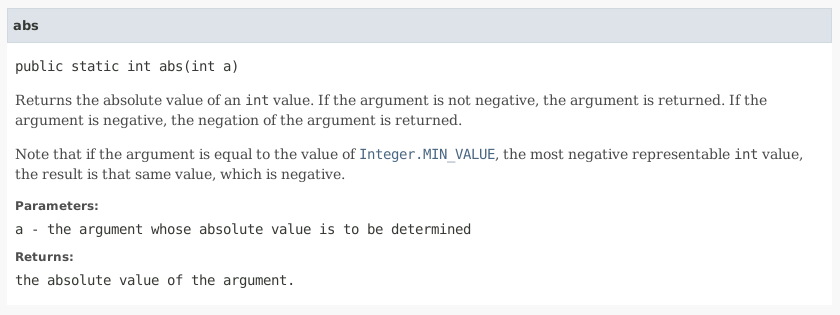
\includegraphics[width=0.91\textwidth]{../img/screenshot-jdk8-javadoc-abs.png}
	\end{flushright}
\end{frame}

%% === Cours de Java
% === Chapitre : Survol 

\subsection{Alternatives (survol)}

\imgfullh{../img/The_choice_by_vallo29.jpg}
{\centering\color{bluepigment}\Large\bf Alternatives}
{http://vallo29.deviantart.com/art/The-choice-150871274}

\begin{frame}[fragile]{Instructions de choix}
Le \emph{Si}
\begin{Java}
  if ( condition ) {
    instructions
  }
\end{Java}
\bigskip
Le \emph{Si-sinon}
\begin{Java}
  if ( condition ) {
    instructions
  } else {
    instructions
  }
\end{Java} 
\end{frame}

\begin{frame}[fragile]{Exemple} 
\begin{Java}
import java.util.Scanner;
public class Test {
  public static void main(String[] args) {
      Scanner clavier = new Scanner(System.in);
      int nombre1;

      nombre1 = clavier.nextInt();
      if (nombre1 < 0) {
         System.out.println(nombre1 + " est n�gatif"); 
      }   
  }
}
\end{Java}
\end{frame}

\begin{frame}[fragile]{Exemple} 
\begin{Java}
import java.util.Scanner;
public class Test {
  public static void main(String[] args) {
      Scanner clavier = new Scanner(System.in);
      int nombre1;

      nombre1 = clavier.nextInt();
      System.out.println(nombre1 + " est un nombre ");
      if (nombre1 < 0) {
         System.out.println("n�gatif"); 
      } else {
         System.out.println("positif");   
      }
  }
}
\end{Java}
\end{frame}

\begin{frame}[fragile]{Exercice} 
Comment traduire cet algorithme ?
\begin{Code}
MODULE test ()
    nombre1: Entier
    LIRE nombre1
    SI nombre1 > 0 ALORS
        ECRIRE nombre1, "est positif"
    SINON
        SI nombre1 = 0 ALORS
            ECRIRE nombre1, "est nul"
        SINON
            ECRIRE nombre1, "est n�gatif"
        FIN SI
    FIN SI
FIN MODULE
\end{Code}
\end{frame}

\begin{frame}[fragile]{Expressions bool�ennes} 
	Les comparateurs
	\begin{center}
		\Large
		\java|<| \; \java|>| \; \java|<=| \; \java|>=| \; \java|==| \; \java|!=|
	\end{center}
	Les op�rateurs bool�ens 
	\begin{center}
		\Large
		\java|&&| (et) \: \java{||} (ou) \: \java|!| (non)
	\end{center}
\end{frame}

\begin{frame}[fragile]{Exemple} 
\begin{Java}
import java.util.Scanner;
public class Exemple {
  public static void main(String[] args) {
      Scanner clavier = new Scanner(System.in);
      int nombre1;

      nombre1 = clavier.nextInt();
      if ((nombre1 % 2) == 0) {
         System.out.println("Le nombre est pair");
      } else {
         System.out.println("Le nombre est impair"); 
      }
  }
}
\end{Java}
\end{frame}

\begin{frame}[fragile]{Exemple} 
\begin{Java}
import java.util.Scanner;
public class Exemple {
  public static void main(String[] args) {
      Scanner clavier = new Scanner(System.in);
      int �ge;

      �ge = clavier.nextInt();
      if ( �ge<21 || �ge>=60 ) {
         System.out.println("Tarif r�duit !");
      }
  }
}
\end{Java}
\end{frame}

\begin{frame}[fragile]{Le \og selon-que\fg} 
Premi�re forme
\begin{Java}
  switch(produit) {
    case "Coca" : 
    case "Sprite" : 
    case "Fanta" :  
        prixDistributeur=60; 
        break;
    case "IceTea" : 
        prixDistributeur=70; 
        break;
    default :       
        prixDistributeur=0; 
        break;
  }
\end{Java}
\begin{itemize}
\item Notez le \java{break}
\item Possible avec : entiers, caract�res et chaines
\end{itemize}
\end{frame}

\begin{frame}[fragile]{Le \og selon-que\fg} 
Deuxi�me forme : la logique suivante
\begin{Code}
  Selon que 
    nb > 0 : �crire "positif"
    nb = 0 : �crire "nul"
    autres : �crire "n�gatif"
  Fin selon que
\end{Code}
s'�crit en Java
\begin{Java}
  if (nb>0) {
      System.out.println("positif");
  } else if (nb==0) {
      System.out.println("nul");
  } else {
      System.out.println("n�gatif");
  }  
\end{Java}
\end{frame}



% ==S�ance 4
\section{Lisibilit� et notions de modules}
\leconwithtocquote
{\og Any fool can write code that a computer can understand.
\\Good programmers write code that humans can understand. \fg
\\Martin Fowler}
% === Cours de Java

\section{�crire du code lisible}

\leconwithabstractquote{Nous montrons pourquoi et comment\\�crire du code lisible}
{\og Any fool can write code that a computer can understand.
\\Good programmers write code that humans can understand. \fg
\\Martin Fowler}

\begin{frame}[fragile]{Et pourtant �a tourne !}
On a vu que le compilateur ne se pr�occupe pas de la \textit{mise en page}
\begin{itemize}
\item Tous les \textit{whitespace} sont �limin�s lors de l'analyse lexicale
(\textit{whitespace} $\equiv$ \textit{espace}, \textit{retour � la ligne}, \dots)
\end{itemize}
$\Longrightarrow$ ceci est \emph{�quivalent} au \textit{Hello World}
\begin{Java}
public
class
Hello{public static void main(String[] args){System.
out.              println( "Bonjour !"         );}}
\end{Java}
\end{frame}

\begin{frame}{Et pourtant �a tourne !}
C'est correct pour le compilateur mais � \emph{proscrire}
\begin{itemize}
\item Un code est \emph{souvent lu}
  \begin{itemize}
  \item Lorsqu'il est �crit / mis au point
  \item Correction de bug 
  \item �volution du code (les besoins changent)
  \end{itemize}
\item Et souvent par des \emph{personnes diff�rentes}
\end{itemize}
\bigskip
$\Longrightarrow$ \emph{La lisibilit� est essentielle}
\end{frame}

\begin{frame}[fragile]{Un code lisible}
\emph{R�gle 1} : \emph{Indenter} correctement son code 
  \begin{itemize}
  \item Pour un aper�u global de la structure du code
  \item Pour rep�rer rapidement la fin d'un \textit{bloc}
  \end{itemize}
\bigskip
\emph{R�gle 2} : Bien choisir le \emph{nom des variables}
\begin{itemize}
\item Ce bout de code est syntaxiquement correct
\item Mais que fait-il ?
\end{itemize}
\begin{Java}
  int u=clavier.nextInt(),n=clavier.nextInt(),
  t=clavier.nextInt();
  double p=u*n*(1+t/100.0);
  System.out.println(p);
\end{Java}
\end{frame}

\begin{frame}[fragile]{Un code lisible}
Nous lui pr�f�rons celui-ci plus lisible :
\begin{Java}                                                 
  double �Payer;
  int prixUnitaire = clavier.nextInt();
  int nombreArticles = clavier.nextInt();
  int tauxTVA = clavier.nextInt();

  �Payer = prixUnitaire * nombreArticles * (1 + tauxTVA/100.0);

  System.out.println(�Payer);
\end{Java}
\end{frame}

\begin{frame}{Un code lisible}
\emph{R�gle 3} : \emph{D�composer} les expressions trop longues
  \begin{itemize}
  \item Une variable interm�diaire peut accroitre la lisibilit� : le nom donne un sens � l'expression
  \item La perte de place m�moire est n�gligeable 
  \\(voire nulle car un compilateur peut optimiser) 
  \item Trop d�composer nuit parfois � la lisibilit� 
  \\(limite floue)
  \\$\Longrightarrow$ importance de l'\emph{exp�rience}
  \end{itemize}
\end{frame}

\begin{frame}[fragile]{Un code lisible}
\emph{Exemple} : reprenons l'exemple du calcul du prix � payer
\begin{Java}
  int prixUnitaireHTVA = clavier.nextInt();
  int nombreArticles = clavier.nextInt();
  int tauxTVA = clavier.nextInt();
  int prixUnitaireTTC = prixUnitaireHTVA * (1 + tauxTVA/100.0);                               
  double �Payer = prixUnitaireTTC * nombreArticles;
\end{Java}
\medskip
\emph{Exemple} : que pr�f�rer de
\begin{Java}
int hypo = Math.sqrt( a*a + b*b );
\end{Java}
\begin{Java}
int aCarr� = a*a;
int bCarr� = b*b;
int hypo = Math.sqrt( aCarr� + bCarr� );
\end{Java}
\end{frame}

\begin{frame}[fragile]{Un code lisible}
\emph{R�gle 4} : Utiliser des \emph{constantes}
\begin{itemize}
\item Rend le code plus lisible
\item Facilite aussi son �volution
\end{itemize}
\begin{Java}                                                 
  final double TAUX_TVA = 0.21;
  double taxe;
  double prix = clavier.nextInt();
  taxe = prix * TAUX_TVA;
  System.out.println(taxe);
\end{Java}
\end{frame}

\begin{frame}[fragile]{Un code lisible}
\emph{Anti-r�gle} : Surcharger de \emph{commentaires}
\begin{itemize}
\item Vient souvent au secours d'un code non lisible
\item Id�alement on utilisera les commentaires
  \begin{itemize}
  \item En d�but de programme, de module
  \item Pour expliquer \emph{ce qu'il fait}
  \item Mais surtout \emph{pas comment} il le fait
  \item cf. \textit{javadoc}
  \end{itemize} 
\end{itemize}
\bigskip
Il y a d'autres r�gles ? Oui !
\begin{itemize}
\item Pour \sigle{Java}, document reprenant les conventions � respecter :
{\scriptsize \code|http://www.oracle.com/technetwork/java/codeconv-138413.html|}
\end{itemize} 
\end{frame}

\begin{frame}{La refactorisation}
\emph{En r�alit�} : On n'�crit pas un code lisible du premier coup !
\\\bigskip
\emph{Refactoriser} = changer le code en vue d'am�liorer sa lisibilit� / son �volutivit� sans changer ce qu'il fait
  \begin{itemize}
  \item \emph{Exemples}
    \begin{itemize}
    \item donner un nom plus explicite � une variable
    \item mieux indenter le code
    \end{itemize}
  \item \emph{Contre-exemples}
    \begin{itemize}
    \item ajouter une fonctionnalit�
    \item r�parer un bug
    \end{itemize}
  \end{itemize}
\end{frame}

\begin{frame}{La refactorisation}
Mais refactoriser c'est toucher � du code qui fonctionne ! 
Ce n'est pas dangereux ?
\\\medskip
\emph{Oui}! $\Longrightarrow$ importance 
  \begin{itemize}
  \item des tests de \emph{non-r�gression} (cf. \sigle{JUnit})
  \item d'un syst�me de \emph{gestion des versions}
  \end{itemize}
\medskip
Pour aller plus loin : Martin Fowler, \\
<<\textit{Refactoring: Improving the design of existing code}>>
\end{frame}


% === Cours de Java
% === Chapitre : Survol 

\subsection{Code modulaire (premier survol)}

\begin{frame}[fragile]{Les variables}
Les types disponibles
\begin{center}
\begin{tabular}{r|l}
En Algorithmique & En  Java \\ \hline
Entier & \java{int} \\ 
R�el & \java{double} \\ 
Chaine & \java{char}, \java{String} \\ 
Bool�en & \java{boolean} \\  
\end{tabular} 
\end{center}
\end{frame}

\begin{frame}[fragile]{Les calculs}
Op�rateurs :
\begin{center}
	\Large
    \java{+} \java{-} \java{*} \java{/} \java{\%}  
\end{center}
\end{frame}

\begin{frame}[fragile]{Variable}
	On peut stocker une valeur, le r�sultat d'un calcul dans une \emph{variable}
	
	\bigskip
	
	\emph{D�claration}\\
\begin{Java}
   typeVariable nomVariable;
\end{Java}

	\begin{itemize}
	\item Exemples :
\begin{Java}
   int nb1;
   String nom;
\end{Java}
	\end{itemize}
\end{frame}


\begin{frame}[fragile]{Variable}
	\emph{Assignation}\\
	Via le symbole \java{=}
	\begin{itemize}
	\item Exemples :
\begin{Java}
   nb1 = 1;
   nb1 = 3+4;
   nom = "Java";
   moyenne = (nombre1 + nombre2) / 2.0;
   d� = Math.random() * 6 + 1
\end{Java}
	\end{itemize}
\end{frame}


\imgfullh{../img/cut_and_fold_by_alltelleringet-d5jmcpu.jpg}
	{
		\begin{flushright}
			\vspace{3.5cm}
			\Large\bf\color{honeydew} D�couper le code
			\vspace{-3.5cm}
		\end{flushright}
		}
	{http://alltelleringet.deviantart.com/art/Cut-and-Fold-335286498}

\note{
	Expliquer pourquoi d�couper le code. Algo a une volont� d'expliquer que ce 
    d�coupage soit \textbf{naturel}. �vitons donc d'�crire des r�gles. 

    L'id�e c'est: r�utilisabilit�, scinder la difficult�, d�verminer, lisibilit�,
    r�partition du travail.

    On aime qu'une m�thode porte un nom explicite, r�solve un probl�me pr�cis et 
    clairement d�fini, qu'elle soit document�e, etc.
	}


\full[bluepigment]{
	\begin{center}
		\Large\color{white}\textbf{Appel} de m�thode
	\end{center}
}

\begin{frame}{Appel d'une m�thode}
Une m�thode est une \emph{boite noire}
\begin{center}
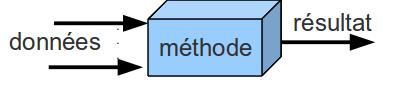
\includegraphics[scale=.6]{../img/methode}
\end{center}
Pour l'utiliser, il faut connaitre\,:
\begin{itemize}
\item son nom;
\item ce dont elle a besoin;
\item ce qu'elle retourne;
\item mais \emph{pas comment} elle fait;
\end{itemize}
\end{frame}

\imgfullh{../img/darkvador-magician.jpg}
{
		\begin{center}
			\color{white}\large
			Pas de \textbf{comment} ? \\
			Un simple \textbf{quoi}
		\end{center}
}
{https://www.flickr.com/photos/st3f4n/14480265204/sizes/l}

\begin{frame}[fragile]{Appel d'une m�thode}
� partir du code d'une \emph{autre classe} 
  \begin{itemize}
  \item \java{NomClasse.nomM�thode(...)}
  \item \emph{Exemples} :
    \begin{Java}
double racine = Math.sqrt(4.0);
double al�atoire = Math.random();
int nb = -10;
int absolu = Math.abs(nb);
    \end{Java}
  \end{itemize}
  \bigskip
  \textit{Un appel de m�thode au sein de la classe ne n�cessite pas de r�p�ter
  le nom de la classe}
\end{frame}

\full[bluepigment]{
	\begin{center}
		\Large\color{azuremist}\textbf{D�finition} d'une m�thode
	\end{center}
}

\begin{frame}[fragile]{D�finition d'une m�thode}
	\textbf{Syntaxe}
	\bigskip
\begin{Java}
public static <typeRetour> <nomM�thode> ([param�tre, param...]) {  
    // instructions
    <return r�sultat>;  
}
\end{Java}
\end{frame}






% ==S�ance 5
\section{Notion de package et survol des structures r�p�titives}
\leconwithtoc


% === Cours de Java

\section{Organiser le code}

\leconwithabstract{Dans une application r�elle, la taille des programmes impose une organisation rigoureuse}

\begin{frame}{Le groupement en package}
L'\emph{API} (Application Programming Interface) d�signe la biblioth�que standard Java
\begin{itemize}
\item Elle contient des \emph{milliers} de classes
\item Elles sont regroup�es en \emph{package}
\end{itemize}
\begin{center}
  %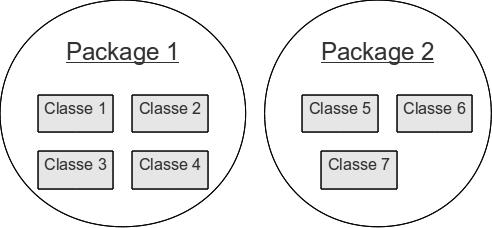
\includegraphics[scale=.6]{../img/package}
\end{center}
\end{frame}

\begin{frame}{La notion de package}
Un \emph{package}
\begin{itemize}
\item Regroupe les classes li�es
\item Permet l'unicit� des noms de classe
  \begin{itemize}
    \item nom complet / qualifi�: {\small \java|monPackage.MaClasse|}
  \end{itemize} 
\end{itemize} 
\bigskip
Nom d'un package
  \begin{itemize}
    \item identifieurs s�par�s par des points \java|.|
    \item tout en minuscules
    \item adresse internet invers�e (unicit�)
    \item ex: {\small \java|be.heb.esi.java1|}, {\small \java|org.apache.struts.action|}
  \end{itemize} 
\end{frame}

\begin{frame}[fragile]{Utilisation}
Pour utiliser une classe 
\begin{itemize}
\item mettre le nom \emph{qualifi�} (complet)
\begin{Java}
  java.util.Calendar now = java.util.Calendar.getInstance();
\end{Java}
\item ou utiliser \java{import} qui cr�e un raccourci
\begin{Java}[basicstyle=\scriptsize]
  import java.util.Calendar;
  public Test {
  ...
    Calendar now = Calendar.getInstance();
  ...
  }
\end{Java}
\item Cas particulier : le package \java|java.lang| est import� implicitement
  \begin{itemize}
  \item Exemple : on peut tout de suite �crire
  \begin{Java}
  double racine = Math.sqrt(1.21);
  \end{Java}
  \end{itemize}
\end{itemize}
\end{frame}

\begin{frame}{Utilisation}
Comment savoir comment utiliser les classes et m�thodes ? En lisant la \emph{javadoc}
%\begin{center}
%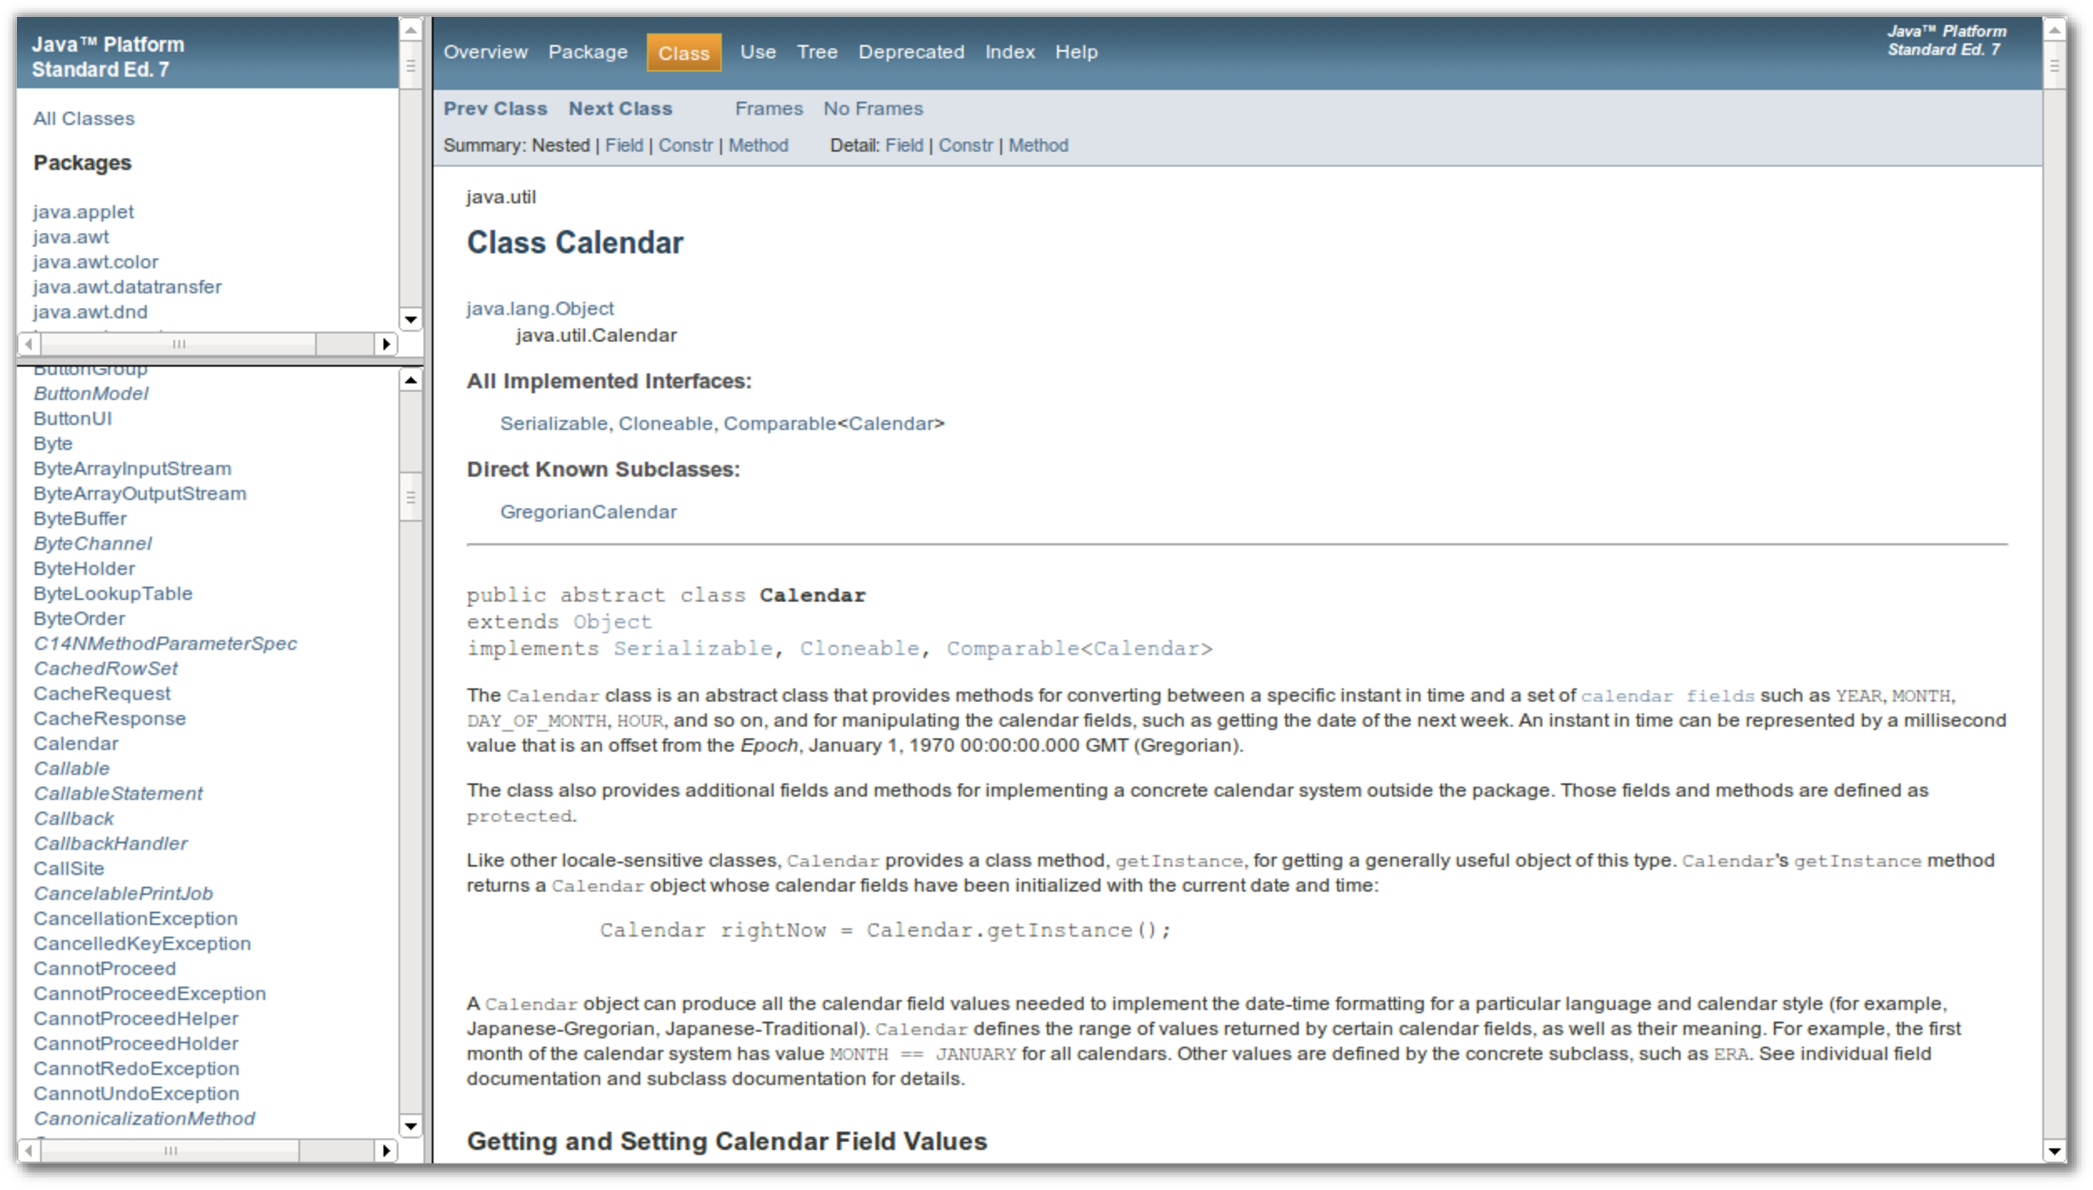
\includegraphics[scale=.28]{../img/api}
%\\ \scriptsize{\textit{(http://download.oracle.com/javase/7/docs/api/)}}
%\end{center}
\end{frame}

\begin{frame}{Utilisation}
On peut y lire le nom du package 
\begin{center}
%
\includegraphics[scale=.6]{../img/api-package}
\end{center}
et la description de la m�thode
%\begin{center}
%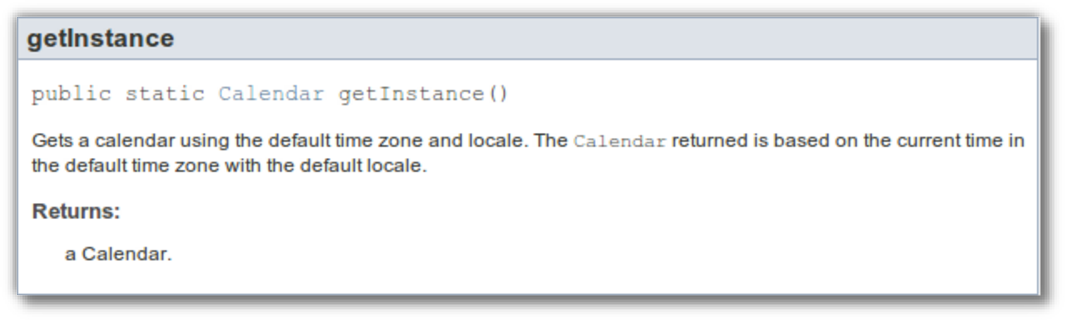
\includegraphics[scale=.6]{../img/api-methode}
%\\{\small \textit{On verra comment produire une \emph{javadoc} similaire pour son code}}
%\end{center}
\end{frame}

\begin{frame}[fragile]{Cr�er ses packages}
Pour placer une classe dans un package, la commande est \java|package nom_package;|
  \begin{itemize}
  \item Doit �tre la \emph{premi�re instruction} du fichier 
  \item Exemple :
\begin{Java}
package be.heb.esi.java1;
public class Test { 
  // Nom complet : be.heb.esi.java1.Test
}
\end{Java}
  \end{itemize}
\end{frame}

\begin{frame}[fragile]{Cr�er ses packages}
Qu'est-ce qui va changer en pratique ?
\begin{itemize}
\item La compilation ne change pas : 
 \begin{Java}
 javac NomClasse.java
 \end{Java}
\item L'ex�cution change : 
 \begin{Java}
 java nomPackage.NomClasse
 \end{Java}
\item Contraintes sur l'endroit o� placer le \emph{bytecode}
  \begin{itemize}
  \item Li� � la notion de \emph{CLASSPATH} 
  \item Sera d�taill� au laboratoire
  \end{itemize}
\end{itemize}
\end{frame}

\begin{frame}{R�utiliser du code}
Si on doit coder quelque chose, c'est \emph{peut-�tre d�j� fait}
\begin{itemize}
\item $\Longrightarrow$ autant le r�utiliser
  \begin{itemize}
  \item Gain de temps
  \item Probablement mieux �crit
  \end{itemize}
\item Importance de \emph{connaitre l'API}
\\(en tout cas les classes principales)
\end{itemize}
\end{frame}



% === Cours de Java
% === Chapitre : Survol des instructions r�p�titives

\subsection{Les boucles (survol)}

\imgfullw{../img/looptheloop}
	{
		\begin{flushright}
			\color{aliceblue}\Large\it
			\vspace{-3cm}
			Loop the loop !\hspace{1cm}
		\end{flushright}
	}
	{https://www.flickr.com/photos/sirispjelkavik/2801926735/sizes/o/}

\begin{frame}[fragile]{Instructions r�p�titives}
Le \emph{Tant que} : 
\begin{Java}
  while ( condition ) {
    instructions
  }
\end{Java} 
\bigskip
\emph{Exemple} :
\begin{Java}
  int puissance = 1;
  while ( puissance < 1000 ) {
    System.out.println(puissance);
    puissance = 2 * puissance;
  }
\end{Java}
\end{frame}

\begin{frame}[fragile]{Exemple} 
\begin{Java}
import java.util.Scanner;
public class Exemple {
  /**
   * Affiche la somme d'entiers positifs entr�s au clavier.
   * S'arr�te d�s qu'une valeur nulle ou n�gative est donn�e.
   * @param args non utilis�
   */
  public static void main(String[] args) {
      Scanner clavier = new Scanner(System.in);
      int nb;
      int somme = 0;
      nb = clavier.nextInt();
      while ( nb > 0 ) {
         somme = somme + nb;
         nb = clavier.nextInt();
      }
      System.out.println(somme);
  }
}
\end{Java}
\end{frame}

\begin{frame}[fragile]{Instructions r�p�titives}
Le \emph{Pour} : 
\begin{Java}
  for ( int i=d�but; i<=fin; i=i+pas ) {
    instructions
  }
\end{Java} 
\bigskip
\emph{Exemple} :
\begin{Java}
  for ( int i=1; i<=10; i=i+1 ) {
    System.out.println(i);
  }
\end{Java}
\end{frame}

\begin{frame}[fragile]{Exemple} 
\begin{Java}
public class Exemple {
  /**
   * Affiche la somme des nombres pairs entre 2 et 100.
   * @param args non utilis�
   */
  public static void main(String[] args) {
      int somme;

      somme = 0;
      for ( int i=2; i<=100; i=i+2 ) {
         somme = somme + i;
      }
      System.out.println(somme);
  }
}
\end{Java}
\end{frame}

\begin{frame}[fragile]{Exemple} 
\begin{Java}
public class Exemple {
  /**
   * Affiche un compte � rebours � partir de 10.
   * @param args non utilis�
   */
  public static void main(String[] args) {

      for ( int i=10; i>=1; i=i-1 ) {
         System.out.println(i);
      }
      System.out.println("Partez !");
  }
}
\end{Java}
\end{frame}

\begin{frame}[fragile]{Instructions r�p�titives}
\java|i++| est un raccourci pour \java|i=i+1|
\\\bigskip
\emph{Exemple} :
\begin{Java}
  for ( int i=1; i<=n; i++ ) {
    System.out.println(i);
  }
\end{Java} 
\end{frame}

\full[bluepigment]{
	\begin{center}
		\Large\bf\color{azuremist}
		�tude de cas\\
		\it
		Lecture d'une donn�e enti�re positive
	\end{center}
}

\begin{frame}[fragile]{�tude de cas} 
\begin{itemize}
\item \emph{�tape 1} : lire un entier
\end{itemize}
\begin{Java}
/**
  * Lit un entier au clavier.
  * Les valeurs non enti�res sont pass�es.
  * @return l'entier lu.
  */
public static int lireEntier() {
    Scanner clavier = new Scanner(System.in);
    int nb;
    // Tant que ce n'est pas un entier au clavier
    while ( !clavier.hasNextInt() ) {
        clavier.next(); // le lire, le passer
    }
    nb = clavier.nextInt();
    return nb;
}
\end{Java}
\end{frame}

\begin{frame}[fragile]{�tude de cas} 
\begin{itemize}
\item \emph{�tape 2} : lire un entier positif
\end{itemize}
\begin{Java}
/**
  * Lit un entier au clavier.
  * Les valeurs non enti�res, nulles ou n�gatives sont pass�es.
  * @return l'entier lu.
  */
public static int lirePositif() {
    int nb;
    nb = lireEntier();
    while (nb<=0) {
      nb = lireEntier();
    }
    return nb;
}
\end{Java}
\end{frame}

\begin{frame}[fragile]{�tude de cas}
	\begin{itemize}
		\item \emph{�tape 3}: un exemple de main
	\end{itemize}
	\begin{Java}
/**
 * Un exemple de main.
 */
 public static void main(String[] args){
	int nombreLu;

	System.out.print("Entre un entier positif: ");
	nombreLu = lirePositif();
 }
	\end{Java}
\end{frame}






% ==S�ance 6
\section{�crire du code robuste, la gestion des erreurs}
\leconwithtoc

% === Cours de Java
\subsection{�crire du code robuste}

\imgfullw{../img/sinking_boat_by_msholly.jpg}{
		\Large\bf\color{aliceblue}
		\vspace{3.5cm}
		Environnement d�faillant
	}
	{http://msholly.deviantart.com/art/sinking-boat-156264295}

\begin{frame}{Motivation}
Un programme ne tourne pas dans un monde id�al
\\\bigskip
Il doit pouvoir \emph{r�sister aux d�faillances} de l'environnement
  \begin{itemize}
  \item On tente d'ouvrir un fichier qui n'existe pas
  \item L'utilisateur entre des donn�es incorrectes
  \item \dots
  \end{itemize}
\end{frame}

\subsection{G�rer les erreurs}

\begin{frame}[fragile]{La gestion des erreurs}
\emph{Exemple} :
\begin{Java}
import java.util.Scanner;
public class Affiche {
  /**
   * Affiche un nombre entier lu au clavier.
   * @param args non utilis�
   */
  public static void main(String[] args) {
      Scanner clavier = new Scanner(System.in);
      int nb;
 
      nb = clavier.nextInt();
      System.out.println(nb);
  }
}
\end{Java}
\end{frame}


\begin{frame}[fragile]{La gestion des erreurs}
Et si l'utilisateur entre une lettre ?
\vspace{-1ex}
\begin{center}
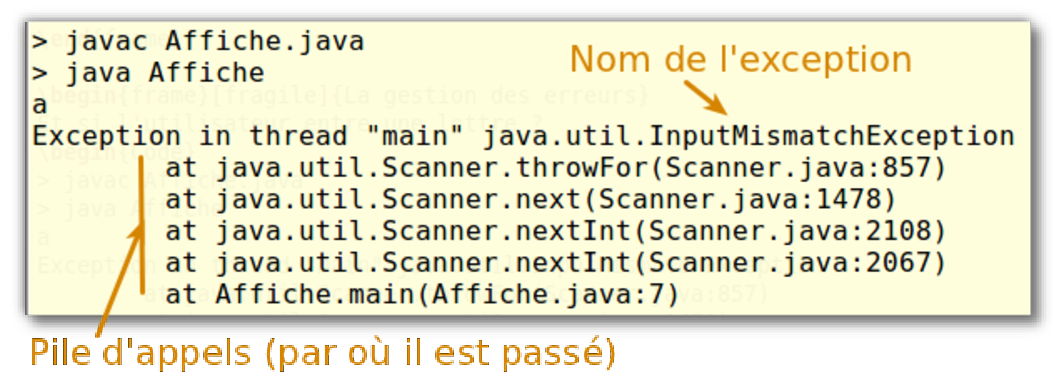
\includegraphics[scale=.65]{../img/erreur1}
\end{center}
\vspace{-1ex}
%\begin{Code}
%> javac Affiche.java
%> java Affiche
%a
%Exception in thread "main" java.util.InputMismatchException
%	at java.util.Scanner.throwFor(Scanner.java:857)
%	at java.util.Scanner.next(Scanner.java:1478)
%	at java.util.Scanner.nextInt(Scanner.java:2108)
%	at java.util.Scanner.nextInt(Scanner.java:2067)
%	at Affiche.main(Affiche.java:7)
%\end{Code}
\end{frame}

\full[bluepigment]{
	\begin{center}
		\color{azuremist}\Large\bf
		Comment (essayer) \\de g�rer le probl�me ? 
	\end{center}
}

\imgfullw{../img/puffinwithcatch}{
	\Huge\bf\color{burntorange}
	\vspace{3cm}
	catch
}
{https://www.flickr.com/photos/47515486@N05/11845113373/sizes/l}


\begin{frame}[fragile]{La gestion des erreurs}
L'instruction \java|try catch|
  \begin{itemize}
  \item \java{try} : contient les instructions qui \emph{peuvent mal se passer}
  \item \java{catch} : contient le code qui est \emph{en charge} de g�rer le probl�me
  \end{itemize}
\bigskip
Quand un probl�me se pr�sente dans le \java{try}
  \begin{itemize}
  \item Le code du \java{try} est interrompu
  \item Le code du \java{catch} est ex�cut�
  \item Ensuite, on continue apr�s le \java{try-catch} 
  \end{itemize}
\end{frame}

\begin{frame}[fragile]{La gestion des erreurs}
\emph{Exemple} : on affiche un message plus clair
\begin{Java}[basicstyle=\scriptsize]
package be.heb.esi.lgj1;
import java.util.Scanner;
public class Affiche {
  /**
   * Affiche l'entier lu au clavier ou un message si ce n'est pas un entier.
   * @param args inutilis�.
   */
  public static void main(String[] args) {
      Scanner clavier = new Scanner(System.in);
      int nb;
      try { 
        nb = clavier.nextInt();
        System.out.println(nb);
      }
      catch(Exception e) { 
        System.out.println("Ce n'est pas un entier!");
      }
  }
}
\end{Java}
\vspace{-4ex}
\hspace{3ex}
%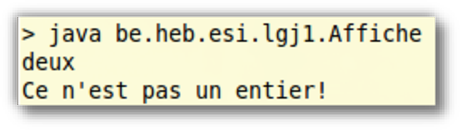
\includegraphics[scale=.65]{../img/throw}
\end{frame}

\subsection{Confiner les probl�mes}

\begin{frame}{Confiner les probl�mes - Motivation}
Imaginons la situation suivante :
\begin{itemize}
\item Un programme demande un entier � l'utilisateur
\item Il doit �tre positif
\item L'utilisateur entre un nombre n�gatif
\item Le programme ne le v�rifie pas tout de suite
\end{itemize}
\end{frame}

\begin{frame}{Confiner les probl�mes - Motivation}
On aura un probl�me :
\begin{itemize}
\item Un plantage
\item Un r�sultat erron�
\item Un effet ind�sir� (perte de donn�es, \dots)
\end{itemize}
\medskip
Mais le probl�me va survenir :
\begin{itemize}
\item Plus tard dans le temps
\item Plus loin dans le code
\end{itemize}
\medskip
$\Longrightarrow$ \emph{Difficile} � comprendre et \emph{corriger}
\end{frame}

\begin{frame}{Confiner les probl�mes}
Besoin de \emph{confiner} les probl�mes
  \begin{itemize}
  \item Un probl�me est \emph{d�tect� rapidement} avant qu'il ne se propage dans le reste du code
  \end{itemize}
\bigskip
Cas pratique : v�rifier les \emph{param�tres}
  \begin{itemize}
  \item Si une contrainte est associ�e � un param�tre
    \begin{itemize}
    \item Le v�rifier en d�but de m�thode
    \item Que faire si pas valide ?
    \end{itemize}
  \end{itemize}
\end{frame}

\full[bluepigment]{
	\begin{center}
		\color{azuremist}\Large\bf
		Lancer une exception
	\end{center}
}


\begin{frame}[fragile]{Confiner les probl�mes}
	\emph{Lancer} une exception
\begin{Java}[basicstyle=\scriptsize]
  /**
   * Calcule la racine carr�e d'un nombre.
   * @param nb le nombre dont on veut la racine car�e.
   * @return la racine carr�e de <code>nb<\code>.
   * @throws IllegalArgumentException si <code>nb</code> est n�gatif.
   */
  public static double racineCarr�e(double nb) {
    if (nb<0) {
      throw new IllegalArgumentException("nb doit �tre positif!");
    }
    // Traitement normal. On est s�r que le param�tre est OK.
  }
\end{Java}
\end{frame}

\begin{frame}[fragile]{Confiner les probl�mes}
\emph{Exemple}
\begin{Java}
  try {
    System.out.println( racineCarr�e( val ) );
  } catch (Exception ex) {
    System.out.println( "Calcul impossible !" );
  }
\end{Java}
\bigskip
On peut aussi pr�ciser qu'on n'attrape \emph{que} les \java|IllegalArgumentException|
\begin{Java}
  try {
    System.out.println( racineCarr�e( val ) );
  } catch (IllegalArgumentException ex) {
    System.out.println( "Calcul impossible !" );
  }
\end{Java}
\end{frame}

%% === Cours de Java
% === Chapitre : Les donn�es

\section{Les types et les litt�raux}

\leconwithtoc

\subsection{Un langage typ�}

\begin{frame}{Les types}
\emph{Toute donn�e a un type}
  \begin{itemize}
  \item Coh�rence s�mantique
  \item Allocation m�moire adapt�e
  \end{itemize}  
\bigskip
Quels types ?
\begin{itemize}
  \item \emph{primitifs pr�d�finis} : 
\begin{itemize}
\item entier, r�el, bool�en (logique)
\end{itemize}
  \item \emph{r�f�rences pr�d�finis} :
\begin{itemize}
\item tableaux, String, \dots
\end{itemize}
  \item \emph{r�f�rences d�finis par le programmeur}
  \end{itemize}
\end{frame}

\begin{frame}[fragile]{Les types primitifs}
\vspace{-25pt}
\begin{center}
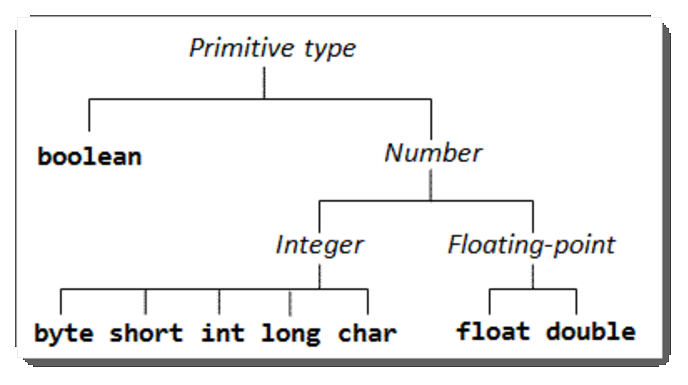
\includegraphics[scale=.65]{../img/primitifs}
\\\tiny{source : http://www3.ntu.edu.sg/home/ehchua/programming/java/J2\_Basics.html}
\end{center}
\vspace{-25pt}
\begin{columns}[T]
\begin{column}{0.5\textwidth}
\begin{grammaire}
\nterm{PrimitiveType} : one of
    \nterm{NumericType}  \term{boolean}

\nterm{NumericType} : one of
    \nterm{IntegralType}  \nterm{FloatingPointType}
\end{grammaire}
\end{column}
\begin{column}{0.4\textwidth}
\begin{grammaire}
\nterm{IntegralType} : one of
    \term{byte}  \term{short}  \term{int}  \term{long}  \term{char}

\nterm{FloatingPointType} : one of
    \term{float}  \term{double}
\end{grammaire}
\end{column}
\end{columns}
\end{frame}

\subsection{Les types entiers}

\begin{frame}[fragile]{Les types num�riques entiers}
\java|byte|, \java|short|, \java|int| et \java|long| 
(\java|char| sera vu � part) :
\begin{itemize}
\item Nombres sign�s (en compl�ment � 2)
\item Cod�s sur 8-bit, 16-bit, 32-bit et 64-bit
\item Comprennent donc les valeurs 
  \begin{itemize}
  \item -128 � 127
  \item -32768 � 32767
  \item -2147483648 � 2147483647
  \item -9223372036854775808 � 9223372036854775807
  \end{itemize} 
\item \emph{Mod�lisation} de la notion math�matique d'entier
  \begin{itemize}
  \item Capacit� limit�e 
  \item permet de repr�senter un intervalle fini de $\mathbb{Z}$
  \item \emph{\textit{out of range}} possible
  \end{itemize} 
\end{itemize}
\end{frame}

\begin{frame}[fragile]{Les litt�raux entiers}
\emph{\textit{Litt�ral}} : repr�sentation d'une valeur
\\\smallskip
Pour les entiers, diff�rents formats sont possibles
\begin{center}
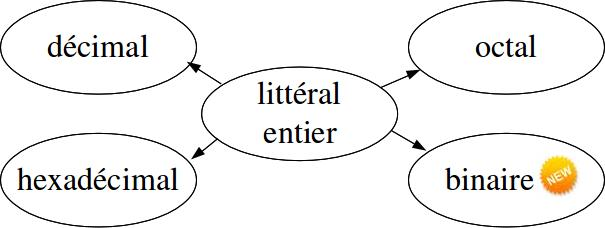
\includegraphics[scale=.35]{../img/java-data-entier}
\end{center} 
\begin{grammaire}
\nterm{IntegerLiteral} : one of
       \nterm{DecimalIntegerLiteral}    \nterm{HexIntegerLiteral}  
       \nterm{OctalIntegerLiteral}        \nterm{BinaryIntegerLiteral}
\end{grammaire}
\end{frame}

\begin{frame}[fragile]{Les litt�raux entiers}
Un \emph{\nterm{DecimalNumeral}} (num�rique d�cimal)  
\vspace{-10pt}
\begin{columns}[T]
\begin{column}{0.6\textwidth}
\begin{grammaire}[fontsize=\footnotesize]
\nterm{DecimalIntegerLiteral} :
     \nterm{DecimalNumeral} \nterm{IntegerTypeSuffix}\opt
\end{grammaire}
\end{column}
\begin{column}{0.4\textwidth}
\begin{grammaire}[fontsize=\footnotesize]
\nterm{IntegerTypeSuffix} : one of \term{l} \term{L}
\end{grammaire}
\end{column}
\end{columns}
  \begin{itemize}
  \item \nterm{DecimalNumeral} : suite de chiffres
  \item \java|_| permis pour la lisibilit� 
\includegraphics[scale=.5]{../img/java7.jpeg} 
  \item Le suffixe (\java|l| ou \java|L|) : distingue un \java|int| d'un \java|long|
  \item Pas de \java|byte| ou \java|short| ? �crire un \java|int|
  \item Pas de \emph{litt�ral n�gatif} ? Utiliser le \java|-|
  \item Exemples corrects : \java|0   1275   1_421   23L| 
  \item Exemples incorrects : \java|12.3   1 000   1,000   1.0| 
  \end{itemize} 
\end{frame}

\begin{frame}[fragile]{Les litt�raux entiers}
\emph{Octal}
  \begin{itemize}
  \item pr�c�d� de \java|0|
  \item chiffres de 0 � 7
  \end{itemize} 
\emph{H�xad�cimal}
  \begin{itemize}
  \item pr�c�d� de \java|0x| ou \java|0X|
  \item chiffres + a,b,c,d,e,f (minuscules/majuscules)
  \end{itemize} 
\emph{Binaire}
  \begin{itemize}
  \item pr�c�d� de \java|0b| ou \java|0B|
  \item chiffres 0 et 1
  \end{itemize} 
\end{frame}

\begin{frame}[fragile]{Les litt�raux entiers}
\emph{Exemple} : Quelques litt�raux corrects pour la quantit� 100 de type \java|int| 
\begin{itemize}
\item \java|100|
\item \java|1_0_0|
\item \java|0144|
\item \java|01_44|
\item \java|0x64|
\item \java|0b110_0100|
\end{itemize} 
\end{frame}

\begin{frame}[fragile]{Le type num�rique caract�re}
\java|char|
\begin{itemize}
\item Caract�re Unicode
\item Entier non sign� sur 16 bits
\item Assimil� � un entier (on peut faire des calculs !)
\item Plusieurs notations  
\begin{grammaire}[commandchars=|()]
|nterm(CharacterLiteral) :
    |term(') |nterm(SingleCharacter) |term(')
    |term(') |nterm(EscapeSequence) |term(')
\end{grammaire} 
\item La plus simple : le \emph{caract�re entre \textit{single quote}} 
\begin{grammaire}[commandchars=|()]
|nterm(SingleCharacter) :
    any character but not |term(') or |nterm(\) or |nterm(LineTerminator)
\end{grammaire} 
\end{itemize}
\end{frame}

\begin{frame}[fragile]{Les litt�raux caract�res}
Notations sp�ciales avec les s�quences d'�chappement (\textit{Escape Sequence})
\begin{itemize}
\item Pour les caract�res non repr�sentables simplement
\\\medskip
\begin{tabular}{r|llr|llr|l}
\java|\n| & line feed       & \hspace{0.3cm} & \java|\t| & tabulation & \hspace{0.3cm} & \java|\'| & \code|'| \\
\java|\r| & carriage return & \hspace{0.3cm} & \java|\b| & backspace  & \hspace{0.3cm} & \java|\"| & \code|"| \\
          &                 & \hspace{0.3cm} &           &            & \hspace{0.3cm} & \java|\\| & \code|\| \\
\end{tabular}
\medskip
\begin{itemize}
\item Exemples : \java|'\n'| ,\java|'\\'| ,\java|'\''|
\end{itemize}
\item Pour utiliser le code Unicode
\begin{itemize}
\item Exemples : 
  \begin{itemize}
  \item \java|'\u0F40'| pour le \textit{KA} tib�tain 
  \item \java|'\u17E0'| pour le chiffre 0 Khmer 
  \end{itemize}
\end{itemize}
\end{itemize}
\end{frame}

\subsection{Les types flottants}

\begin{frame}[fragile]{Les types � virgule flottante}
\java|float|, \java|double| 
\begin{itemize}
\item Respectent la norme IEEE754
\item Cod�s sur (respectivement) 32-bit, et 64-bit
\item On utilisera plus souvent le type \java|double|
\item \emph{Mod�lisation} de la notion math�matique
  \begin{itemize}
  \item Capacit� limit�e (\emph{\textit{out of range}} possible) 
  \item Pr�cision limit�e
    \begin{itemize}
    \item $\longrightarrow$ \emph{impr�cision} lors d'un calcul
    \item ex : $10^{-30}$ est repr�sentable et pourtant \\$(1+10^{-30})-1$ donnera $0$ et pas $10^{-30}$
    \end{itemize}
  \end{itemize} 
\end{itemize}
\end{frame}

\begin{frame}[fragile]{Les litt�raux � virgule flottante}
Notation assez souple
\begin{grammaire}
\nterm{FloatingPointLiteral} :
      \nterm{Digits} \term{.} \nterm{Digits}\opt \nterm{ExponentPart}\opt \nterm{FloatTypeSuffix}\opt
      \term{.} \nterm{Digits} \nterm{ExponentPart}\opt \nterm{FloatTypeSuffix}\opt
      \nterm{Digits} \nterm{ExponentPart} \nterm{FloatTypeSuffix}\opt
      \nterm{Digits} \nterm{ExponentPart}\opt \nterm{FloatTypeSuffix}

\nterm{ExponentPart} :
      \term{e} \nterm{signedInteger}
      \term{E} \nterm{signedInteger}

\nterm{FloatTypeSuffix} : one of
      \term{f} \term{F} \term{d} \term{D}
\end{grammaire}
\end{frame}

\begin{frame}[fragile]{Les litt�raux � virgule flottante}
\begin{small}
\begin{tabular}{|c|c|c|c|c|c|}
\hline
partie enti�re & . & partie d�cimale & E & exposant & suffixe \\
\hline
\end{tabular}
\end{small}
\smallskip
\begin{itemize}
\item 4 parties optionnelles (mais pas ensemble)
\begin{itemize}
\item Cela doit rester sens�
\item On ne peut pas le confondre avec un entier
\end{itemize}
\item En l'absence de suffixe : un double
\item Exemples : \java|1.2E3|, \java|1.F|, \java|.1|, \java|1e-2d|, \java|1f|
\item Contre-exemples : \java|1|, \java|.E1|, \java|E1|
\end{itemize}
\end{frame}

\subsection{Les bool�ens}

\begin{frame}{Le type bool�en}
\java|boolean|
\begin{itemize}
\item Appel� aussi \emph{logique}
\item 2 valeurs : \java|true| (vrai) et \java|false| (faux)
\end{itemize}
\end{frame}

\subsection{La chaine de caract�res}

\begin{frame}[fragile]{La chaine de caract�res}
\java|String|
\begin{grammaire}[commandchars=|()]
|nterm(StringLiteral) :
      |term(") |nterm(StringCharacters)|opt |term(")
|nterm(StringCharacters) :
      |nterm(StringCharacter)
      |nterm(StringCharacters) |nterm(StringCharacter)
|nterm(StringCharacter) :
      |nterm(InputCharacter) but not |term(") or |term(\)
      |nterm(EscapeSequence)
|nterm(InputCharacter) :
      |nterm(UnicodeInputCharacter) but not |term(CR) or |term(LF)
\end{grammaire}
\begin{itemize}
\item Exemples de \java|String| :
\begin{itemize}
\item \java|"Bonjour "|
\item \java|"'Un peu de tout' : \"\n\\"|
\end{itemize} 
\item Attention : \java|char| $\neq$ \java|String|
\end{itemize}
\end{frame}





% ==S�ance 7
\section{La javadoc}
\leconwithtocquote{%
	\og  It's not a bug - it's an undocumented feature. \fg%
	\\Author Unknown}

% === Cours de Java
% === Chapitre : Javadoc
\subsection{La documentation}

\imgfullw{../img/explosion-paint.jpg}{
	\Large\bf\color{white}
	\vspace{-3.9cm}
	La documentation
}{}

\note{
	\par La documentation, une touche de couleur qui ne � sert � rien � \ldots
	mais qui change tout ! 
}

%%%
%\%subsubsection{Motivation}

\begin{frame}{Motivation}
	\begin{center}
		\Large\bf\color{bluepigment}
		\par Pour qui ?
		\par Qu'�crire ?
	\end{center}
\end{frame}

\note{
	\begin{itemize}
		\item Pour qui ?
		\begin{itemize}
			\item Le programmeur qui va \emph{utiliser} le code
			\item Le programmeur qui va \emph{maintenir} le code \\(peut-�tre vous)
		\end{itemize}
		\item Quel type de documentation ?
		\begin{itemize}
			\item \emph{Ce que fait} la m�thode/classe
			\item \emph{Comment} elle le fait
			\\(peut �tre r�duit au minimum si code lisible)
		\end{itemize}
	\end{itemize}
}

\note{
	Qui est int�ress� par quoi ?
	\begin{itemize}
		\item Le programmeur-\emph{utilisateur}
		\begin{itemize}
			\item int�ress� uniquement par le \emph{quoi}
		\end{itemize}
		\item Le programmeur-\emph{mainteneur}
		\begin{itemize}
			\item int�ress� par le \emph{quoi} et le \emph{comment}
		\end{itemize}
	\end{itemize}
}

\begin{frame}{Motivation}
	\textbf{O� mettre la documentation ?}
	\bigskip
	\begin{itemize}
		\item Avec le code
		\begin{itemize}
			\item Plus facile pour le maintenir
			\item Plus de chance de garder la synchronisation avec le code
		\end{itemize}
		\item Mais le programmeur-utilisateur n'a pas � voir le code pour l'utiliser
		\end{itemize}
\end{frame}

\begin{frame}{Motivation}
	
\includegraphics[width=51px]{../img/icon_15706}
   	\emph{litterate programming}
   	\medskip
   	\begin{itemize}
		\item la documentation accompagne le code
		\item un outil extrait cette documentation pour en faire un document facile � lire
		\item toute la documentation suit la m�me structure, le m�me style
\\$\rightarrow$ plus facile � lire
	\end{itemize}
\end{frame}

%%%
\subsection{javadoc}

\imgfullh{../img/mur-cerisierjapon-9580504952_080b2591db_o.jpg}{
	\begin{center}
		\color{white}\Large\bf
		code $\xrightarrow{ javadoc  }$ doc
	\end{center}
}{}

\begin{frame}[fragile]{Javadoc}
	\sigle{\bf javadoc}
	\begin{itemize}
		\item Commentaire \sigle{javadoc} identifi� par  {\small \code|/** ... */|}
\begin{Java}
/**
    Calcule et retourne le maximum de 2 nombres.
*/
\end{Java}
		\item documentation produite au format \sigle{HTML}
		\item On commente essentiellement 
		\begin{itemize}
			\item la classe: r�le et fonctionnement
			\item les m�thodes publiques: ce que �a fait, param�tres et r�sultats
		\end{itemize}
		\item Se met \emph{juste au dessus} de ce qui est comment�
	\end{itemize}
\end{frame}

\subsection{Les tags}

\begin{frame}{Les tags}
	Utilisation de \emph{tags} pour identifier certains �l�ments
	\\\bigskip 
	Les plus courants :
	\begin{itemize}
		\item \emph{@param} : d�crit les param�tres 
		\item \emph{@return} : d�crit ce qui est retourn�
		\item \emph{@throws} : sp�cifie les exceptions lanc�es 
		\item \emph{@author} : note sur l'auteur
	\end{itemize}
\end{frame}

\begin{frame}[fragile]{Les tags}
\emph{Exemple}
\begin{Java}
/**
 * Donne la racine carr�e d'un nombre.
 * @param nb le nombre dont on veut la racine carr�e.
 * @return la racine carr�e du nombre.
 * @throws IllegalArgumentException si le nombre est n�gatif.
*/
public static double sqrt( double nb ) {...}
\end{Java}
\begin{itemize}
\item Les types sont d�duits de la signature et ajout�s � la documentation
\item La premi�re phrase (termin�e par un \java|.|) sert de r�sum�
\end{itemize}
\end{frame}

\begin{frame}{Les tags}
R�sum�
\vspace{-10pt}
\begin{center}
	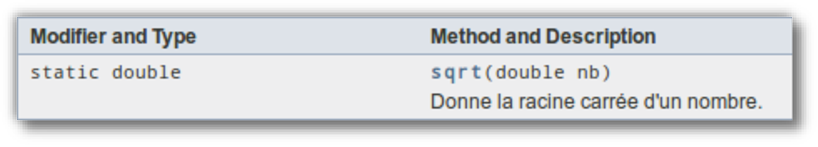
\includegraphics[scale=.6]{../img/javadoc-resume}
\end{center}
\vspace{-10pt}
D�tail
\vspace{-10pt}
\begin{center}
	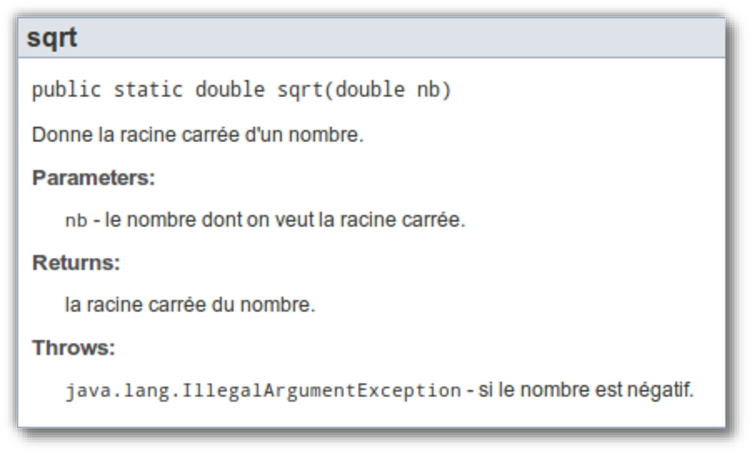
\includegraphics[scale=.6]{../img/javadoc-detail}
\end{center}
\end{frame}

%\subsubsection{Le code HTML}

\begin{frame}[fragile]{Le code HTML}
	Peut contenir des balises \sigle{HTML}
	\\\medskip
\emph{Exemple} :
\begin{Java}[basicstyle=\scriptsize]
  /**
  * Indique si l'ann�e est bissextile. Pour rappel :
  * <ul>
  *   <li>Une ann�e qui n'est pas divisible par 4 n'est pas bissextile 
  *       (ex: 2009)</li>
  *   <li>Une ann�e qui est divisible par 4</li>
  *     <ul>
  *     <li>est en g�n�ral bissextile (ex: 2008)</li>
  *     <li>sauf si c'est un multiple de 100 mais pas de 400 (ex: 1900, 2100)</li>
  *     <li>les multiples de 400 sont donc bien bissextiles (ex: 2000, 2400)</li>
  *     </ul>
  *   </ul>
  * Plus formellement, <code>a</code> est bissextile si et seulement si <br/>
  * <code>a MOD 400 = 0 OU (a MOD 4 = 0 ET a MOD 100 != 0)</code>
  * @param ann�e l'ann�e dont on se demande si elle est bissextile 
  * @return vrai si l'ann�e est bissextile
  */
\end{Java}
\end{frame}

\begin{frame}{Le code HTML}
	Ce qui donne
\begin{center}
	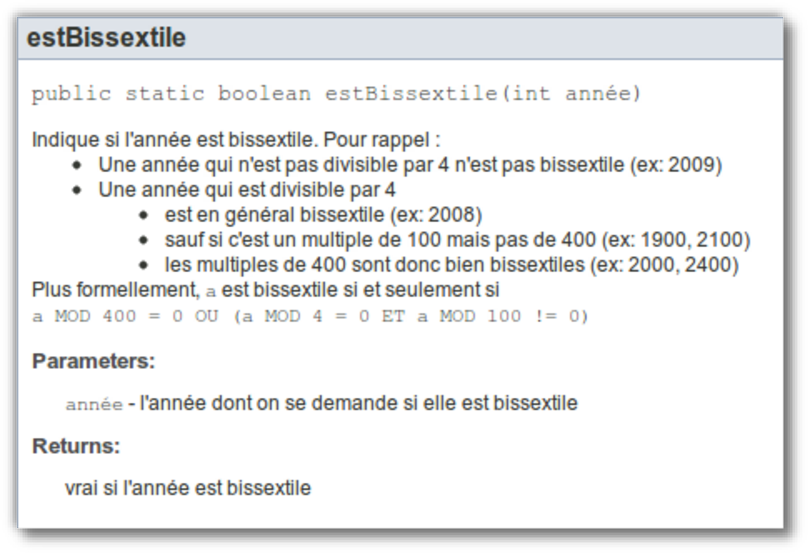
\includegraphics[scale=.7]{../img/javadoc-html}
\end{center}
\end{frame}

%%%
%\subsubsection{Produire la documentation}

\begin{frame}[fragile]{Production de la documentation}
	Commande \code|javadoc|
	\begin{itemize}
		\item \java|javadoc Temps.java|
		\item \java|javadoc *.java|
		\item \java|javadoc -d doc *.java |
		\item \java|javadoc -charset utf-8 *.java |
		\item \ldots et beaucoup d'autres options
		\\(cf. documentation de \sigle{javadoc})
	\end{itemize}
\end{frame}

%%%
%\subsubsection{Pour une <<bonne>> documentation}

\begin{frame}{Une bonne documentation}
	Une bonne \textit{javadoc} d�crit le \emph{quoi} mais jamais le \emph{comment}
	\begin{itemize}
	\item $\longrightarrow$ Ne jamais parler de ce qui est priv�
	\item Mauvais exemples :
	\begin{itemize}
		\item \textit{On utilise un for pour parcourir le tableau.}
  		\item \textit{Pour aller plus vite, on stocke le prix hors tva dans 
  			une variable temporaire.}
  	\end{itemize}
	\end{itemize}
\end{frame}

\begin{frame}[fragile]{Une bonne documentation}
	Ne pas �crire ce que \sigle{javadoc} �crit lui-m�me :
	\begin{itemize}
		\item Mauvais exemples :
  		\begin{itemize}
  			\item \textit{nb - un entier qui ...}
  			\item \textit{La m�thode sqrt ...}
  			\item \textit{Cette m�thode ne retourne rien.}
  		\end{itemize}
	\item Pour en savoir plus :
{\scriptsize \url{http://www.oracle.com/technetwork/articles/java/index-137868.html}}
\end{itemize}
\end{frame}


%%%
\subsection{�tude de cas}
\full[bluepigment]{
	\begin{center}
		\Large\bf\color{azuremist}
		\href{http://thenounproject.com/term/consultation/39938/}{%
			
\includegraphics[width=50px]{../img/icon_39938_transwhite.png}}
		\par\bigskip
		�tude de cas
	\end{center}
}


% ==S�ance 9
\section{Le survol des tableaux}
\leconwithtoc

% === Cours de Java

\subsection{Les tableaux (survol)}

\begin{frame}{Avertissement}
	\begin{center}
		Nous pr�sentons ici une vue \emph{simplifi�e} 
		\\des tableaux en Java afin de \emph{coller} 
		\\� votre cours d'\emph{algorithmique}.
		\bigskip
		\\Nous aurons l'occasion d'�tre plus pr�cis 
		\\lors d'une prochaine le�on.
\end{center}
\end{frame}

\imgfullh{../img/color-bucket-12641657814_c8de7afa1e_k.jpg}{
	\begin{center}
		\bf\LARGE\color{azuremist}
		tableau\\
		\medskip
		\Large
		plusieurs variables de m�me type
	\end{center}
}{https://www.flickr.com/photos/michel_poitrenaud/12641657814}

\begin{frame}[fragile]{Pr�sentation}
	\par N�cessit� de manipuler \emph{plusieurs variables similaires} auxquelles 
	on acc�de par un \emph{indice}
  	\begin{center}
		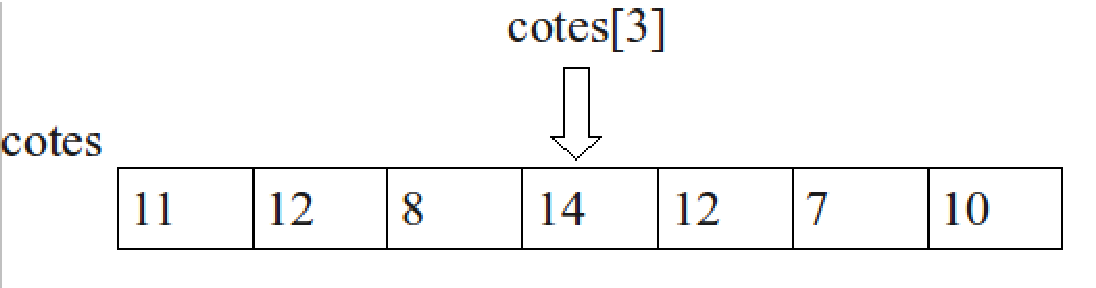
\includegraphics[scale=.35]{../img/tab-pres}
	\end{center}
	\bigskip
	Pourquoi pas plusieurs variables ?
\end{frame}

\note{
	\begin{itemize}
		\item \emph{Ex}: plusieurs cotes, plusieurs temp�ratures
		\item Acc�s � un des �l�ments via un \emph{indice} (\textit{position})
	\end{itemize}
}

\begin{frame}[fragile]{Pr�sentation}
	\par �criture \emph{compacte} et qui s'\emph{adapte} � la taille
	\bigskip
	\par \emph{Exemple} 
	\par En algorithmique, si \java|tableau| est un tableau de $N$ entiers
     \begin{Java}
  pour i de 0 � N-1 faire
     afficher tableau[i]
  fin pour
     \end{Java}
\end{frame}


%%%
%\subsubsection{D�claration / Cr�ation}

\full[bluepigment]{
	\Huge\tt\bf\color{brickred}
	[]
	\par\vspace{2cm}
	\LARGE\bf\color{azuremist}
	D�claration
	\bigskip
	\Large\tt
	\par Type[] identifier
}

\begin{frame}[fragile]{D�claration}
	\emph{Exemples}
    \begin{itemize}
    	\item \java|int[]| est le type \textit{tableau d'entiers}
	    \item \java|String[]| est le type \textit{tableau de chaines de caract�res}
    \end{itemize}
	\bigskip
	\bigskip
    \begin{Java}
    int[] cotes;
    String[] noms;
    \end{Java}
\end{frame}

\note{
	En \sigle{Java} : uniquement des tableaux \emph{dynamiques}
    \begin{itemize}
    	\item La taille ne fait pas partie du type
	    \item D�claration et cr�ation sont s�par�es
    \end{itemize}
	La d�claration suit la syntaxe habituelle
}

\full[bluepigment]{
	\Huge\tt\bf\color{brickred}
	new
	\par\vspace{2cm}
	\LARGE\bf\color{azuremist}
	Cr�ation
	\bigskip
	\Large\tt
	\par identifier = new Type[taille]	
}


\begin{frame}[fragile]{Cr�ation}
	\emph{Exemple}
	\begin{itemize}
		\item new int[3]
		\item new String[taille] o� taille est d�fini
	\end{itemize}
	\bigskip
    \begin{Java}
    int[] entiers;
    entiers = new int[3];
    \end{Java}
    \bigskip
	\emph{Remarque}
	\\La d�claration et la cr�ation peuvent �tre combin�es
    \\\java|int[] entiers = new int[3];|
\end{frame}

\full[bluepigment]{
	\Huge\tt\bf\color{brickred}
	\{\}
	\par\vspace{2cm}
	\LARGE\bf\color{azuremist}
	Initialisation
	\bigskip
	\Large\tt
	\par identifier = new Type[] \{x, x\}	
}

\begin{frame}[fragile]{Initialisation}
	\emph{Exemple}
	\begin{itemize}
		\item new int[] \{42, 17, -5\}
		\item new String[] \{"foo", "bar"\}
	\end{itemize}
	\bigskip
	\begin{Java}
		int[] entiers = new int[] {0x2A, 021, -5};
		String[] noms = new String[] 
		    {"Victoria", "Melanie", "Melanie",  "Emma", "Geri"};

		double[] r�els;
		r�els = new double[] {4.2, -1};
	\end{Java}
	\bigskip
	\small{
	\emph{Remarque}
	\\Par d�faut, les �l�ments sont initialis�s � \java|0| (num�riques) 
	ou \java|false| (bool�ens)
}
\end{frame}

\begin{frame}[fragile]{Cr�ation et initialisation}
	\emph{Cas particulier}
	\par
	Cr�ation du tableau et initialisation en une seule �tape, 
	\\en \emph{donnant ses valeurs}
	\vspace{1cm}
    \begin{Java}
		int[] entiers = {0x2A, 021, -5};
		double[] pseudoR�els = {4.5, 1E-4, -4.12, Math.PI};

		double[] r�els;
		r�els = {4.2, -1}; // FAUX
    \end{Java}
\end{frame}


%\subsubsection{Acc�s}

\imgfullh{../img/a_bath_in_a_bucket.jpg}{
	\Large\bf\color{snow}
	\vspace{2.5cm}
	Acc�s aux �l�ments
	\par\vspace{5mm}\color{brickred}\texttt{\Huge\bf[i]}
}{http://n-scapephotography.deviantart.com/art/A-bath-in-a-bucket-286676419}

\begin{frame}[fragile]{Acc�s aux �l�ments}
	\emph{\huge\bf [i]}
	\begin{itemize}
  		\item 0 est l'indice de d�part
		\item indices de \emph{0} � \emph{taille du tableau - 1}
		\item la taille du tableau est son nombre d'�l�ments
  	\end{itemize}
  	\bigskip
    \begin{Java}
    int[] entiers = {3, 14, 15};
    int entier = entiers[2]; // entier vaut 15
    entiers[1] = 85;
    entier = 0;
    entier = entiers[entier+1]; //entier vaut 85
    \end{Java}
\end{frame}

\begin{frame}[fragile]{Acc�s aux �l�ments}
  \emph{Exemple}
  \medskip
  \begin{Java}
  package be.heb.esi.lg1.tutorials.tableaux;

  public class InitialisationTableau {
     public static void main(String[] args) {
        int[] entiers = new int[10];
        for(int i = 0; i < 10; i++) {
           entiers[i] = i;
        }
     }
  }
  \end{Java}
\end{frame}

%%%
%\subsubsection{Taille}

\imgfullh{../img/plantationmai-2013-bw.jpg}{
	\begin{flushright}
		\begin{minipage}[l]{.4\linewidth}
			\color{brickred}
			Un tableau connait 
			\\\textbf{\Large sa taille}
			\bigskip
			\\\color{black}\texttt{identifier.length}
		\end{minipage}
	\end{flushright}
}{home made � la plantation du mai 2013}

\begin{frame}[fragile]{Taille}
  \emph{Exemple}
  \bigskip
  \begin{Java}
  int[] entiers = {4, 5, 6};
  int taille = entiers.length;
  System.out.println(taille); // �crit 3
  \end{Java}
\end{frame}

\begin{frame}[fragile]{Taille}
  	\emph{Exemple}
  	\bigskip
  	\begin{Java}
  package be.heb.esi.lg1.tutorials.tableaux;

  public class SimpleParcoursAscendant {
     public static void main(String[] args){
        int[] entiers = {1, 2, 3, 4, 5, 6, 7, 8, 9, 10};
        for(int i = 0; i < entiers.length; i = i + 1) {
           System.out.println(entiers[i]);
        }
     }
  }
  \end{Java}
\end{frame}

\begin{frame}[fragile]{Taille}
  	\emph{Exemple}
  	\bigskip
  	\begin{Java}
  package be.heb.esi.lg1.tutorials.tableaux;

  public class SimpleParcoursDescendant {
     public static void main(String[] args){
        int[] entiers = {1, 2, 3, 4, 5, 6, 7, 8, 9, 10};
        for(int i = entiers.length - 1; i >= 0; i = i-1) {
           System.out.println(entiers[i]);
        }
     }
  }
  \end{Java}
\end{frame}


%%%
%\subsubsection{Tableau et m�thode}

\begin{frame}[fragile]{Tableau et m�thode}
Un tableau peut �tre un param�tre d'une m�thode.
\\\emph{Exemple} : Afficher un tableau 
\begin{Java}
   public static void afficher( int[] entiers ) {
      for(int i = 0; i<entiers.length; i++) {
         System.out.println(entiers[i]);
      }
   }
\end{Java}
\begin{itemize}
  \item L'appel pourrait �tre
  \begin{Java}
  int[] cotes = {12, 8, 10, 14, 9};
  afficher( cotes );
  \end{Java}
\end{itemize}
\end{frame}

\begin{frame}[fragile]{Tableau et m�thode}
	\begin{center}
		En \sigle{Java}, \textbf{passage de param�tre par valeur}. 
		\par\bigskip
		Pour un tableau, cela signifie que l'on ne peut pas \\
		modifier le tableau dans son ensemble mais que \\
		l'on pourra modifier ses �l�ments.
 	\end{center}
\end{frame}

\begin{frame}[fragile]{Tableau et m�thode}
  \emph{Exemple}
  \begin{Java}
   public static void remplir( int[] entiers, int val ) {
      for(int i = 0; i<entiers.length; i++) {
         entiers[i] = val;
      }
   }
  \end{Java}
  \begin{itemize}
  	\item L'appel pourrait �tre
  \begin{Java}
  int[] cotes = new int[16]; // Ne pas oublier de le cr�er
  remplir( cotes, 20 );
  \end{Java}
  \end{itemize}
\end{frame}

\begin{frame}[fragile]{Tableau et m�thode}
 	\emph{Exemple}
 	\begin{Java}
    public static void m�thodeFausse( double[] r�els) {
        double[] r�elsDePassage = {4.2, -7, Math.PI};
        r�els = r�elsDePassage; // INUTILE
   }
 	\end{Java}
 	\bigskip
 	Quel que soit l'appel, le tableau que l'on passe en param�tre ne sera pas
 	modifi�
\end{frame}

\note{
	\par Diff�rencier passage de param�tre par valeur et en entr�e-sortie. 
	Comparer la situation en algorithmique et en java
}

\begin{frame}[fragile]{Tableau et m�thode}
  Un tableau peut �tre une valeur de retour
  \\\emph{Exemple} : Cr�er un tableau avec valeur
  \begin{Java}
   public static int[] cr�er( int taille, int val ) {
      int[] entiers = new int[taille];
      for(int i = 0; i<taille; i++) {
         entiers[i] = val;
      }
      return entiers;
   }
  \end{Java}
  \begin{itemize}
  \item L'appel pourrait �tre
  \begin{Java}
  int[] cotes = cr�er(16, 20);
  \end{Java}
  \end{itemize}
\end{frame}

\subsection{Erreurs fr�quentes}

\begin{frame}[fragile]{Erreurs fr�quentes}
	\textbf{Exceptions}
	\begin{itemize}
		\item \java|NullPointerException| : si vous essayez d'acc�der � un �l�ment d'un tableau qui n'a pas �t� cr��
		\\(le tableau vaut \java|null| dans ce cas)
		\item \java|ArrayIndexOutOfBoundsException| : si vous donnez un indice qui n'existe pas (ex: \java|tab[10]| quand il n'y a que 10 �l�ments dans le tableau)
	\end{itemize}
\end{frame}




% ==S�ance 9
\section{Variables locales}
\leconwithtocquote{\og  The best performance improvement is the transition 
from the nonworking state to the working state. \fg\ J. Osterhout}

% === Cours de Java
% === Chapitre : Les donn�es
%%%
%\section{Variables locales}

%%%
%\subsection{Pr�sentation}

\imgfullh{../img/Phangan__s_bucket__by_tiboudmiss.jpg}{
	\color{white}\bf\Large
	\vspace{-1.5cm}
	Variable locale
}{http://tiboudmiss.deviantart.com/art/Phangan-s-bucket-163211431}

\begin{frame}{Pr�sentation}
	D�signation g�n�rique d'un \emph{emplacement} de la \emph{m�moire vive}
	\begin{itemize}
		\item \emph{Poss�de un type}
		\item Ne peut contenir que des valeurs de ce type
		\item Allocation diff�rente si type \\\emph{primitif} ou \emph{r�f�rence}
	\end{itemize}
\end{frame}

%%%
\subsection{Allocation m�moire}

\begin{frame}{Allocation m�moire}
	Pour un type \emph{primitif}
	\begin{itemize}
		\item Indique la zone m�moire (sur la pile/{\it stack}) 
			o� se trouve la \emph{valeur}
	\end{itemize}
	\vspace{-1ex}
	\begin{center}
		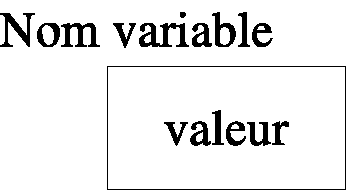
\includegraphics[scale=.4]{../img/java-data-primitive} 
	\end{center}
\end{frame}

\begin{frame}{Allocation m�moire}
	Pour un type \emph{r�f�rence} (ex: \java|String|, tableau)
	\begin{itemize}
		\item La zone m�moire contient l'\emph{adresse} de la zone m�moire 
			(sur le tas/{\it heap}) contenant la valeur (indirection)
	\end{itemize} 
	\begin{center}
		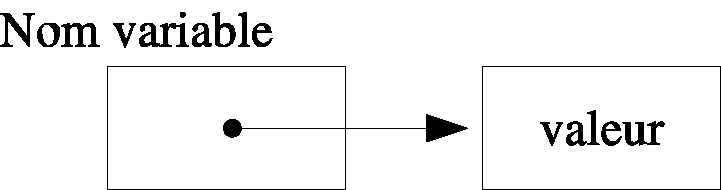
\includegraphics[scale=.4]{../img/java-data-reference} 
	\end{center}
\end{frame}

%%%
\subsection{D�claration}

\begin{frame}[fragile]{D�claration}
	Une varibale d�clar�e dans un \emph{bloc} \ldots 
	\\\hspace{1cm}est locale � ce \emph{bloc}		
	\bigskip
	\begin{grammaire}
	\nterm{Block} :
    \term{\{} \nterm{BlockStatements}\opt \term{\}}

	\nterm{BlockStatement} :
    \nterm{LocalVariableDeclarationStatement}
    \nterm{Statement}
	\end{grammaire}
\end{frame}

\begin{frame}[fragile]{D�claration}
	\textbf{D�claration}
	\par 
	\verb$<type> <identifier> [= expression]$
	\bigskip
	\par
	\emph{Exemples} :
	\begin{itemize}
		\item \java|int i;|
		\item \java|String nom, pr�nom;|
		\item \java|boolean ok=true, fini;|
		\item \java|char lettre, chiffre='1';| 
	\end{itemize}
\end{frame}


%%%
\subsection{Conventions sur les noms}

\begin{frame}{Nom d'une variable}
	\textbf{\textit{Identifier}}
	\par\bigskip
	Quel nom peut-on choisir ? 
	\begin{itemize}
  		\item R�gles \sigle{Java}
			\\\textit{javaletter}, \$,\_, \sout{1}
  		\item Conventions 
			\\\textit{mixedCase}, noms explicites
  	\end{itemize}
	\begin{flushright}
		\LARGE\bf\color{brickred} \$ \_ \,
	\end{flushright}
\end{frame}

\note{
	R�gles \emph{impos�es} par la grammaire
	\begin{itemize}
		\item Longueur illimit�e
		\item Compos� de \textit{lettres}, de \textit{chiffres}, 
			\java|$| et \java|_| %$
		\\(internationalisation)
		\item Ne commence pas par un chiffre
		\item $\neq$ \nterm{keyword} ou \nterm{litteral}
		\item Ex valides : \java|nom|, \java|Nom|, \java|Nom23|, 
			\java|Unpeu2touT|%$
		\item Ex invalides : \java|2main|, \java|le total|, \java|for|, 
			\java|true|, \java|12|
	\end{itemize}	
}

\note{
	Conventions \emph{suppl�mentaires}
	\begin{itemize}
		\item Utilis�es dans le monde entier
		\begin{itemize}
			\item Eviter \java|$| et \java|_| %$
			\item Commence par une minuscule
			\item Plusieurs mots accoll�s $\Rightarrow$ les suivants commencent par une majuscule ({\it mixedcase})
			\item Noms explicites (sauf abr�viations courantes)
			\item Articles omis
		\end{itemize} 
		\item Autres recommandations de \sout{\sigle{Sun}} \sigle{Oracle}
		\begin{itemize}
			\item D�clarer en d�but de bloc
			\item Une d�claration par ligne
		\end{itemize} 
	\end{itemize}
}


%%%
\subsection{Valeur initiale}

\begin{frame}[fragile]{Valeur initiale}
	\textbf{Initialisation}
	\par\medskip
	\begin{itemize}
		\item Par d�faut les variables \emph{ne} sont \emph{pas} initialis�es
		\item N'importe quelle expression calculable � cet endroit l� (� l'ex�cution)
	\end{itemize}
\end{frame}


\begin{frame}[fragile]{Valeur initiale}
	\textbf{Exemple}
	\begin{Java}
int poidsKilo = 20; // Un poids en kilos
int poidsGramme = 1000*poidsKilo; // L'�quivalent en grammes
	\end{Java}  
	\medskip
	\begin{Java}
int poidsKilo; // Un poids en kilos
int poidsGramme = 1000*poidsKilo; // erreur � la COMPILATION
	\end{Java}  
\end{frame}

%%%
\subsection{Le concept de <<port�e>>}

\begin{frame}{Scope (port�e) d'une variable locale}
	\textbf{D�finition} Le \emph{\textit{scope}} (\emph{port�e}) d'une 
	variable indique la portion du programme o� elle \textit{existe}
	\par\bigskip
	Le \textit{scope} d'une variable locale est
	\begin{itemize}
		\item le \textit{block} de sa d�claration (entre \java|\{\}|)
		\item d�s sa propre initialisation
	\end{itemize} 
\end{frame}

\begin{frame}[fragile]{Scope (port�e) d'une variable locale}
	\emph{Exemples} : bon ou pas ?
\begin{Java}
{
   int x = y; 
   int y = 1;
}
\end{Java}
\begin{Java}
{
   int x;
   int y = x; 
}
\end{Java}
\begin{Java}
{
  int x = 1, y = x; 
}
\end{Java}
\end{frame}

%%%
\subsection{Constantes}

\begin{frame}[fragile]{Constante}
	\par
	{\large \java|final|}
	\par\bigskip
	Valeur donn�e
	\begin{itemize}
		\item Soit � la d�claration 
		\item Soit par assignation ult�rieure
	\end{itemize} 
	\bigskip
	\begin{Java}
  final int X = 1;
  final int Y;
  Y = 2*X;
  X = 2; // Erreur : poss�de d�j� une valeur
  Y = 3; // Idem
	\end{Java}
\end{frame}

\begin{frame}[fragile]{Constante}
Convention de nom diff�rente
\begin{itemize}
\item Tout mettre en \emph{majuscules}
\item Utiliser \java|_|  pour s�parer les mots
\end{itemize} 
\emph{Exemples}
\begin{Java}
  final double PI = 3.1415;
  final int TAUX_TVA = 21;
\end{Java}
\end{frame}




%% === Cours de Java
% === Chapitre : La grammaire
\section{La notion de grammaire}

\leconwithtoc

\subsection{La notion de grammaire}

\begin{frame}{Le besoin d'une r�f�rence}
	Un langage de programmation doit pouvoir
		\begin{itemize}
		\item \emph{�tre d�crit} aupr�s des programmeurs
		\item faire l'objet d'une \emph{compilation rigoureuse}
		\end{itemize} 
	\medskip\pause
	Il faut un \emph{document de r�f�rence}
		\begin{itemize}
		\item Pour Java : \emph{The Java Language Specification}
			\begin{itemize}
			\item Contient beaucoup de texte (en \emph{Anglais})
				\\ parfois \emph{incomplet} / \emph{ambigu}
			\item N�cessit� d'utiliser un \emph{formalisme} pr�cis : 
				\\ une \emph{grammaire} 
			\end{itemize} 
		\end{itemize} 
\end{frame}

\begin{frame}{Analogie avec le fran�ais}
	Le fran�ais aussi doit pouvoir �tre d�crit
	\begin{center}
		phrase $\supset$ mots $\supset$ caract�res
	\end{center} 
	\begin{itemize}
		\item
			L'\emph{alphabet} donne les caract�res reconnus
		\item 
			Un \emph{dictionnaire/lexique} donne les mots corrects
		\item 
			La \emph{grammaire} renseigne sur l'ordre des mots
		\item 
			La \emph{s�mantique} traite du sens de la phrase
		\item Exemples :
			\\\textit{<<L$\epsilon$ ch$\wedge\uparrow$ $\bowtie$>>}
			\hfill\textit{<<El tahc tse rion>>} 
			\\\textit{<<Le est chat noir>>} 
			\hfill\textit{<<La table boit la t�l�>>}
	\end{itemize}
\end{frame}

\begin{frame}{Un langage de programmation}
	Qu'en est-il pour un langage de programmation ?
	\begin{itemize}
		\item
			L'alphabet : liste donn�e dans la r�f�rence
		\item 
			Les mots (\emph{token} en informatique)
			\begin{itemize}
				\item Impossible via un dictionnaire. Pourquoi ?
				\item Donn�s par une \emph{grammaire lexicale}
			\end{itemize}
		\item 
			Les s�quences de mots : donn�es par une \emph{grammaire syntaxique}
		\item 
			La \emph{s�mantique} : ne peut �tre d�crite formellement
	\end{itemize}
\end{frame}

\begin{frame}{La notion de grammaire}
	Grammaire
		\begin{itemize}
		\item Description \emph{finie} de l'\emph{infinit�} des programmes corrects
		\item Compos�e de
			\begin{itemize}
			\item l'ensemble des tokens pouvant apparaitre tels quels (\textit{symboles \emph{terminaux}})
			\item l'ensemble des \emph{r�gles de production}
				\begin{itemize}
				\item nom de la r�gle (\textit{symbole \emph{non terminal}})
				\item s�quences de symboles produits par la r�gle 
				\end{itemize}
			\item une r�gle de production de \emph{d�part} 
			\end{itemize}
		\end{itemize}
		\begin{center}
		Est \emph{valide} ce qui peut �tre \emph{produit} par la grammaire
		\end{center}
\end{frame}

\begin{frame}{La notion de grammaire}
	La grammaire \emph{lexicale} valide les tokens 
		\begin{itemize}
		\item les symboles terminaux sont les caract�res
		\item les r�gles construisent le mot 
		\end{itemize}
	\bigskip
	La grammaire \emph{syntaxique} valide les s�quences de tokens 
		\begin{itemize}
		\item les symboles terminaux sont les mots
		\item les r�gles construisent la phrase 
		\end{itemize}
\end{frame}

\begin{frame}[fragile]{Exemple : le langage MU}
Inventons un nouveau langage : le \emph{langage MU}
\begin{itemize}
\item Nous devons indiquer de mani�re pr�cise quelle phrase est valide dans notre langage
\item Cela se fait en donnant sa grammaire
\pause
  \begin{itemize}
  \item Les 3 symboles terminaux: \texttt{M},\texttt{U},\texttt{I}
  \item Les 3 r�gles de production
  \begin{small}
\begin{verbatim}
  start:
       debut MU fin

  debut:                   fin:
       debut I                I fin
       I                      I 
\end{verbatim}
  \end{small}
  \item La r�gle de d�part : \texttt{start}
  \end{itemize}
\end{itemize}
\end{frame}


\begin{frame}{Exemple : le langage MU}
Quelques \emph{phrases correctes} (qu'on peut \textit{produire}) 
  \begin{itemize}
  \item \texttt{IMUI}
  \item \texttt{IIMUI}
  \item \texttt{IMUIIIIIIIIIIIIIIIIIIIIIIIII}
  \item \dots � l'infini
  \end{itemize} 
\medskip \pause
Quelques \emph{phrases incorrectes} (impossibles � \textit{produire}) 
  \begin{itemize}
  \item \texttt{MU}
  \item \texttt{MUI}
  \item \texttt{MUIMU}
  \item \dots � l'infini
  \end{itemize} \end{frame}

\begin{frame}[fragile]{Exemple}
Voici un autre exemple
\begin{itemize}
\item Le symbole terminal: \texttt{A}
\item Les 2 r�gles de production
\begin{verbatim}
  liste:
       element
       element liste
  element:
       A  
\end{verbatim}
\item La r�gle de d�part : \texttt{liste}
\end{itemize}
\bigskip
Quel est le langage produit par cette grammaire ?
\end{frame}

\subsection{Notations de la grammaire \sigle{Java}}

\begin{frame}[fragile]{Notations de la grammaire \sigle{Java}}
Une r�gle de la grammaire syntaxique java:
\begin{grammaire}
\nterm{ReturnStatement} :
     \term{return} Expression\opt;
\end{grammaire}
\begin{itemize}
\item Imaginez des exemples d'instruction \og return\fg\ valides
\end{itemize}
\bigskip
La \emph{grammaire compl�te} de \sigle{Java} 
peut �tre consult�e dans le livre
\textit{\og The Java Language Specification\fg}
\end{frame}

%% === Cours de Java
% === Chapitre : La grammaire
\section{La grammaire lexicale de Java}

\leconwithtoc

\subsection{Analyse lexicale}

\begin{frame}{Analyse lexicale de Java}
 Premi�re phase d'analyse d'un programme
\begin{itemize}
\item Examine la s�quence des caract�res d'entr�e
\item Supprime \texttt{caract�res d'espacement} et \texttt{commentaires}
\item Identifie les \textit{tokens} (mots) du langage 
\end{itemize} 
\begin{center}
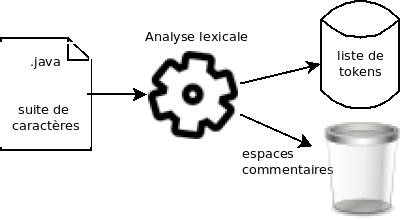
\includegraphics[scale=.5]{../img/phase1} 
\end{center} 
\end{frame}

\begin{frame}{Analyse lexicale de Java}
L'analyse lexicale se base sur une grammaire lexicale
\begin{itemize}
\item Les symboles \texttt{terminaux} sont l'ensemble des caract�res \sigle{Unicode}
\end{itemize} 
\bigskip
\sigle{Java} a fait le choix de l'\sigle{UTF-16} (\sigle{Unicode})
  \begin{itemize}
  \item \sigle{ASCII}: 7 bits
  \item \sigle{ASCII �tendu}: 8 bits
  \item \sigle{EBCDIC}: 8 bits (\sigle{IBM})
  \item \sigle{UTF-16}: 2 bytes, 16 bits 
\\(les 128 premiers caract�res $\equiv$ \sigle{ASCII}) 
  \end{itemize}
\end{frame}

\begin{frame}[fragile]{Les s�quences Unicode}
Java permet une repr�sentation \sigle{ASCII} de tout caract�re \sigle{UTF-16} (via un \textit{caract�re d'�chappement})
\begin{itemize}
\item \emph{Ex} : le caract�re \emph{p} peut aussi s'�crire \code{\u0070} 
\item Une traduction pr�alable est r�alis�e :
\end{itemize}
\begin{Java}
\u0070ublic class MaClasse
\end{Java}
devient
\begin{Java}
public class MaClasse
\end{Java}
\end{frame}

\begin{frame}[fragile]{Les caract�res d'entr�e}
\begin{grammaire}
\nterm{UnicodeInputCharacter} :
   \nterm{UnicodeEscape}
   \nterm{RawInputCharacter}

\nterm{UnicodeEscape} :
   \term{\textbackslash}\nterm{UnicodeMarker} \nterm{HexDigit} \nterm{HexDigit} \nterm{HexDigit} \nterm{HexDigit}

\nterm{UnicodeMarker} :
   \term{u}
   \nterm{UnicodeMarker} \term{u}

\nterm{RawInputCharacter} :
   any Unicode character

\nterm{HexDigit} : one of
   \term{0}  \term{1}  \term{2}  \term{3}  \term{4}  \term{5}  \term{6}  \term{7}  \term{8}  \term{9}    \term{a}  \term{b}  \term{c}  \term{d}  \term{e}  \term{f}     \term{A}  \term{B}  \term{C}  \term{D}  \term{E}  \term{F}  
\end{grammaire}
\end{frame}

\subsection{Les espaces}

\begin{frame}[fragile]{Les caract�res d'espacement}
Les <<espaces>> n'ont pas de sens en \sigle{Java}
\begin{itemize}
\item Peuvent �tre utilis�s librement entre les mots
\item Mais ne peuvent pas couper un mot
\item Exception : les chaines (\textit{String})
\end{itemize}
\begin{grammaire}[basicstyle=\scriptsize]
\nterm{WhiteSpace} :
   the ASCII SP character, also known as "space"
   the ASCII HT character, also known as "horizontal tab"
   the ASCII FF character, also known as "form feed" 
   \nterm{LineTerminator}

\nterm{LineTerminator} :
   the ASCII LF character, also known as "newline"
   the ASCII CR character, also known as "return"
   the ASCII CR character followed by the ASCII LF character
\end{grammaire} 
\end{frame}

\subsection{Les commentaires}

\begin{frame}[fragile]{Le commentaire}
  \begin{itemize}
  \item Sur 1 ligne
    \begin{Java}
// Commentaire sur 1 ligne
    \end{Java}
  \item Sur plusieurs lignes
    \begin{Java}
/* Exemple de commentaire
   sur plusieurs lignes */
    \end{Java}
    \begin{Java}
/** Pour un commentaire Javadoc */
    \end{Java}
  \item Ne peuvent pas �tre imbriqu�s
  \item N'importe o� \textbf{entre} les mots  
  \end{itemize}
\end{frame}

\subsection{Les tokens}

\begin{frame}[fragile]{Les tokens (mots du langage)}
Les caract�res qui restent vont former les \textit{tokens} (mots, symboles terminaux)
\begin{itemize}
\item 5 sortes de tokens 
\begin{grammaire}
\nterm{Token} : one of
    \nterm{Identifier}  \nterm{Literal}  \nterm{Keyword}  \nterm{Separator}  \nterm{Operator}
\end{grammaire}
\end{itemize}
\end{frame}

\begin{frame}[fragile]{Les tokens (mots du langage)}
Liste des \nterm{keyword} (\emph{mots-cl�s} ou r�serv�s)
\begin{grammaire}
\nterm{Keyword} : one of
   \term{abstract}   \term{boolean}   \term{break}   \term{byte}   \term{case}   \term{catch}   
   \term{char} \term{class}   \term{const}   \term{continue}   \term{default}   \term{do}   
   \term{double}   \term{else} \term{extends}   \term{final}   \term{finally}   \term{float}   
   \term{for}   \term{goto}   \term{if} \term{implements}   \term{import}   \term{instanceof}    
   \term{int}   \term{interface} \term{long}   \term{native}   \term{new}   \term{package}   
   \term{private}   \term{protected} \term{public}   \term{return}   \term{short}   
   \term{static}  \term{super}   \term{switch} \term{synchronized}  \term{this}   \term{throw}   
   \term{throws}   \term{transient} \term{try}   \term{void}   \term{volatile}   \term{while}
\end{grammaire}
\end{frame}

\begin{frame}[fragile]{Les tokens (mots du langage)}
Les identifiants
\begin{grammaire}
\nterm{Identifier} :
   \nterm{IdentifierChars} 
         but not a \nterm{Keyword} or \nterm{BooleanLitteral} or \nterm{NullLitteral}

\nterm{IdentifierChars} :
   \nterm{JavaLetter} 
   \nterm{IdentifierChars} \nterm{JavaLetterOrDigit}

\nterm{JavaLetter} :
   any Unicode character that is a Java letter (_ et \$ sont compris)

\nterm{JavaLetterOrDigit} :
   any Unicode character that is a Java letter-or-digit 
\end{grammaire}
(cf. la grammaire compl�te pour les d�tails)
\end{frame}

\begin{frame}[fragile]{Les tokens (mots du langage)}
Liste des s�parateurs et op�rateurs
\begin{grammaire}
\nterm{Separator} : one of
    \term{(}  \term{)}  \term{\{}  \term{\}}  \term{[}  \term{]}  \term{;}  \term{,}  \term{.}

\nterm{Operator} : one of
    \term{=}   \term{>}   \term{<}   \term{!}   \term{~}   \term{?}   \term{:}  \term{==}   \term{<=}   \term{>=}   \term{!=}   \term{&&}   \term{||}   
    \term{++}   \term{--}   \term{+}   \term{-}   \term{*}   \term{/}   \term{&}   \term{|}   \term{^}   \term{%}   \term{<<}   \term{>>}   \term{>>>}
    \term{+=}   \term{-=}   \term{*=}   \term{/=}   \term{&=}   \term{|=}   \term{^=}   \term{%=}   \term{<<=}   \term{>>=}   \term{>>>=}
\end{grammaire}
Comment l'analyseur lexical va-t-il reconnaitre \java|---| ?
\end{frame}

\begin{frame}{R�capitulatif des phases de compilation}
Une fois les tokens identifi�s, le compilateur peut passer � l'analyse syntaxique et s�mantique
\begin{center}
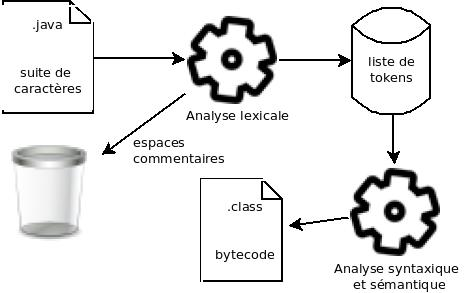
\includegraphics[scale=.5]{../img/phases} 
\end{center} 
\end{frame}



%% === Cours de Java
% === Chapitre : Les expressions

%\section{Les expressions}
\subsection{Les expressions}

\imgfullh{../img/expression_by_bogdanboev-d5rs94g.jpg}{
	\Large\bf\color{white}
	Expression
}{http://bogdanboev.deviantart.com/art/Expression-348998704}

\full[bluepigment]{
	\color{azuremist}
	\textbf{Expression}
	\par\medskip
	Calcul faisant intervenir une ou plusieurs valeur(s) pour une op�ration 
	d�termin�e. 
	\\Cette valeur peut, elle-m�me �tre une expression.
}

\begin{frame}[fragile]{D�finitions}
	\emph{Exemple} : \java|1+2|
  	\begin{itemize}
		\item \java|1| et \java|2| sont les \textbf{op�randes}
		\item \java|+| est l'\textbf{op�rateur}
  		\item l'expression est de type \java|int|
  		\item la valeur de l'expression est $3$
  	\end{itemize}
\end{frame}


%%%
%\subsection{Les expressions enti�res}

\begin{frame}[fragile]{Les expressions enti�res}
	\emph{Op�rateurs}
	\begin{center}
		\Large
		\java$+$ \java$-$
		\hspace{5mm}
		\java$+$ \java$-$ \java$*$ \java$/$ \java|%|
	\end{center}
	\medskip
	\emph{Op�randes} pouvant intervenir
	\begin{itemize}
		\item un \emph{litt�ral} 
		\item une \emph{variable}
		\item une \emph{expression}
	\end{itemize}
\end{frame}

%@todo

\note{
	\par Distinguer les op�rateurs binaires et les unaires 
}


\begin{frame}[fragile]{Les expressions enti�res}
Uniquement avec des op�randes d'un \emph{m�me} type entier
\begin{itemize}
\item Type de l'expression = celui de ses op�randes
\item Exemples :
  \begin{itemize}
  \item \java|1 + 2| vaut $3$ de type \java|int| 
  \item \java|1L + 2L| vaut $3$ de type \java|long| 
  \item \java|3 / 2| vaut $1$ de type \java|int| 
  \end{itemize}
\end{itemize}
\end{frame}

\begin{frame}[fragile]{Priorit� et associativit�}
Probl�me avec l'expression : \java|i + i * 2|
  \begin{itemize}
  \item Le compilateur va-t-il comprendre
    \begin{itemize}
    \item \java|(i+i) *2| ?
    \item \java|i+ (i*2)| ?
    \end{itemize} 
  \end{itemize} 
\bigskip
La strat�gie d'�valuation se base sur
  \begin{itemize}
  \item la \emph{priorit�} d'un op�rateur
  \item l'\emph{associativit�} des op�rateurs de m�me priorit�
  \end{itemize} 
\begin{center}
\begin{tabular}{r|c|c}
 priorit� & op�rateur & associativit� \\ \hline
grande & \java|-|, \java|+| unaires & $\Longleftarrow$ \\
 & \java|*|, \java|/|, \java|%| & $\Longrightarrow$ \\
faible & \java|-|, \java|+| binaires & $\Longrightarrow$ \\
\end{tabular}
\end{center}
\end{frame}

\begin{frame}[fragile]{Tableau des priorit�s et associativit�s}
\emph{Exercices} : comment comprendre
  \begin{itemize}
  \item \java|3 + 3 * 2 + 1| ?
  \item \java|3 + 3 * 2 / - 4 + 5 % 8| ?
  \end{itemize}  
\bigskip
\emph{Parenth�ses} pour forcer la strat�gie 
  \begin{itemize}
  \item Exemple : \java|(3 + 3) * (2 + 1)| $\rightarrow$ \java|6 * 3|  $\rightarrow$ \java|18|
  \end{itemize}
\bigskip
Moralit�: mieux vaut parenth�ser compl�tement
  \begin{itemize}
  \item \emph{ordre explicite} de l'�valuation 
  \item \emph{clart�} pour les autres utilisateurs
  \end{itemize} 
\end{frame}

\begin{frame}{Erreurs de calcul}
La \emph{division par z�ro} 
\begin{itemize}
\item Lance une \textit{exception} (\textit{ArithmeticException})
\item Pour l'instant, \emph{arr�te le programme} avec un message explicite
\end{itemize} 
\bigskip
Le \emph{d�passement de capacit�} 
\begin{itemize}
\item N'est \emph{pas d�tect�} par la machine virtuelle
\item Le r�sultat est tout simplement faux
\end{itemize} 
\end{frame}

\subsection{Les expressions flottantes}

\begin{frame}[fragile]{Les expressions flottantes}
Uniquement avec les op�randes d'un m�me type \emph{flottant}
\begin{itemize}
\item Type de l'expression = type des op�randes
\item Op�rateurs unaires : \java|+| et \java|-|
\item Op�rateurs binaires : \java|+|, \java|-|,\java|*|, \java|/|
\item Le reste est identique aux entiers
\end{itemize}
\smallskip
\emph{Exemples} : Donner la valeur et le type de 
\begin{itemize}
\item \java|1.0 + 2.3| 
\item \java|1.0d - 2.3d|
\item \java|7.0f / 3.5f|  
\item \java|1. / 3.|
\end{itemize} 
\end{frame}

\subsection{Les expressions caract�res}

\begin{frame}[fragile]{Les expressions caract�res}
\java|char| est un type num�rique entier
\begin{itemize}
\item \emph{Aucun op�rateur} sp�cifique 
\item On pourrait effectuer des calculs mais non recommand�
  \\\emph{Exemple} : \java|'a' + 'b'|
\end{itemize}
\end{frame}

\subsection{Les chaines de caract�res}

\begin{frame}[fragile]{Les chaines de caract�res}
Un seul op�rateur (binaire) disponible :
  \begin{itemize}
  \item \java|+| : concat�nation de deux chaines
  \item \emph{Ex} : \java|"Ja"| + \java|"va"| vaut \java|"Java"|
  \end{itemize}
\bigskip
Conversion si un des 2 op�randes n'est pas une chaine.
  \begin{itemize}
  \item \emph{Ex} : \java|""+3.5| vaut \java|"3.5"|
  \item \emph{Ex} : \java|"1"+2+3| vaut \java|"123"|
  \item \emph{Ex} : \java|1+"2"+3| vaut \java|"123"|
  \item \emph{Ex} : \java|1+2+"3"| vaut \java|"33"| !
  \end{itemize}
\end{frame}

\subsection{Les expressions bool�ennes}

\begin{frame}[fragile]{Les expressions bool�ennes}
Op�rateurs :
\begin{itemize}
\item unaire : \java|!| (non)
\item binaires : \java|&&| (et) et \java{||} (ou)
\end{itemize}
\begin{center}
\begin{tabular}{r|c|c}
 priorit� & op�rateur & associativit� \\ \hline
grande & \java|-|, \java|+| unaires, \java|!| & $\Longleftarrow$ \\
 & \java|*|, \java|/|, \java|%| & $\Longrightarrow$ \\
 & \java|-|, \java|+| binaires & $\Longrightarrow$ \\
 & \java|&&| & $\Longrightarrow$ \\
faible & {\color{blue!70!black} \verb,||,} & $\Longrightarrow$ \\
\end{tabular}
\end{center}
\end{frame}

\begin{frame}[fragile]{Les expressions bool�ennes}
\java|&&| : table de v�rit� \\
\medskip
\begin{center}
\begin{tabular}{c|c|c|} 
(ET) & \java|true| & \java|false| \\ \hline
\java|true| & \java|true| & \java|false| \\ \hline
\java|false| & \java|false| & \java|false| \\ \hline
\end{tabular} 
\end{center}
\medskip
Particularit� : si l'op�rande de gauche est \emph{faux}, l'op�rande droit \emph{ne sera pas �valu�} et le r�sultat sera \java|false| 
\end{frame}

\begin{frame}[fragile]{Les expressions bool�ennes}
\java{||} : table de v�rit� \\
\begin{center}
\begin{tabular}{c|c|c|} 
(OU) & \java|true| & \java|false| \\ \hline
\java|true| & \java|true| & \java|true| \\ \hline
\java|false| & \java|true| & \java|false| \\ \hline
\end{tabular} 
\end{center}
\medskip
Particularit� : si l'op�rande de gauche est \emph{vrai}, l'op�rande droit \emph{ne sera pas �valu�} et le r�sultat sera \java|true| 
\end{frame}

\begin{frame}[fragile]{Exemples}
Comment �valuer ?
\begin{itemize}
\item \java{true && false || true} 
\item \java{false || false && ! true} 
\item \java{true || false && true} 
\item \java{false && (true || false)} 
\item \java{!(true || false) && true} 
\end{itemize} 
\end{frame}

\begin{frame}[fragile]{R�sum�}
Voici les r�gles qui r�sument tout ceci
\begin{grammaire}
\nterm{Expression} :
    \nterm{ConditionalOrExpression}

\nterm{ConditionalOrExpression} :
    \nterm{ConditionalAndExpression}
    \nterm{ConditionalOrExpression}  \term{||} \nterm{ConditionalAndExpression}

\nterm{ConditionalAndExpression} :
    \nterm{AdditiveExpression}
    \nterm{ConditionalAndExpression} \term{&&} \nterm{AdditiveExpression}

\nterm{AdditiveExpression} :
    \nterm{MultiplicativeExpression}
    \nterm{AdditiveExpression} \term{+} \nterm{MultiplicativeExpression}
    \nterm{AdditiveExpression} \term{-} \nterm{MultiplicativeExpression}
\end{grammaire} 
\end{frame}

\begin{frame}[fragile]{R�sum�}
\begin{grammaire}
\nterm{MultiplicativeExpression} :
    \nterm{UnaryExpression}
    \nterm{MultiplicativeExpression} \term{*} \nterm{UnaryExpression}
    \nterm{MultiplicativeExpression} \term{/} \nterm{UnaryExpression}
    \nterm{MultiplicativeExpression} \term{%} \nterm{UnaryExpression}

\nterm{UnaryExpression} :
    \term{+} \nterm{UnaryExpression}
    \term{-} \nterm{UnaryExpression}
    \term{!} \nterm{UnaryExpression}
    \nterm{Literal}
    \term{(} \nterm{Expression} \term{)}
    \nterm{Identifier}
\end{grammaire} 
\begin{itemize}
\item On y voit la priorit� et l'associativit� des op�rateurs
\item Pas suffisant pour int�grer toutes les contraintes additionnelles (par exemple ?)
\end{itemize} 
\end{frame}

\subsection{Les expressions relationnelles}

\begin{frame}[fragile]{Les expressions relationnelles}
Op�rateurs de comparaison et d'�galit�
\begin{itemize}
\item Op�randes doivent �tre de \emph{m�me type}
\item Le \emph{r�sultat} est du type \emph{boolean}
\end{itemize} 
\bigskip
Op�rateurs de \emph{comparaison} : {\small \java|<|,\java|>|,\java|<=| et \java|>=|}
  \begin{itemize}
  \item Uniquement pour des \emph{types num�riques} 
  \item Exemple : \java|true < false| n'est pas accept�
  \item Exemple : \java|"Absolu" < "Relatif"| non plus 
  \end{itemize} 
\end{frame}

\begin{frame}[fragile]{L'�galit� de valeurs}
Op�rateurs d'\emph{�galit�} : \java|==| et \java|!=|
  \begin{itemize}
  \item S'appliquent � \emph{tous les types}
  \item Exemple : \java|true == false| est \java|false|
  \item Sens diff�rent si type primitif ou r�f�rence
  \end{itemize}
\bigskip
Type primitif : les \emph{valeurs} sont compar�es
\begin{center}
%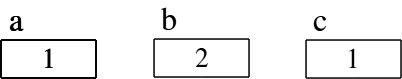
\includegraphics[scale=.5]{../img/java-logi-egal1} 
\end{center}
On a : \java|a==c| mais \java|a!=b| et \java|b!=c|
\end{frame}

\begin{frame}[fragile]{�galit� de valeurs}
Type r�f�rence : les \emph{r�f�rences} sont compar�es
\begin{center}
%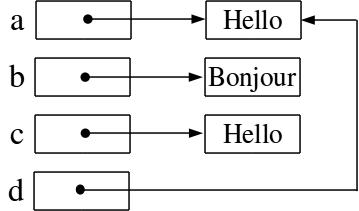
\includegraphics[scale=.5]{../img/java-logi-egal2} 
\end{center}
On a : \java|a!=b|, \java|a!=c| mais \java|a==d|
\end{frame}

\begin{frame}[fragile]{Particularit� du type String}
\begin{Java}
{
  String s1 = "Hello";
  String s2 = "Hello";
  String s3 = "Hel";
  s3 = s3 + "lo";
  System.out.println(s1==s2); // Vrai
  System.out.println(s1==s3); // Faux
  s2 = "Bye";
  System.out.println(s1==s2); // Faux
}
\end{Java}
\begin{itemize}
\item R�utilisation de l'espace mais pour les litt�raux uniquement
\item Pas si r�sultat d'un \emph{calcul} ou \emph{lecture} au clavier
\end{itemize}
\end{frame}

\begin{frame}[fragile]{Egalit� de valeur}
Pour les types r�f�rences, on peut aussi utiliser la m�thode \java|equals| 
\begin{itemize}
\item Ne teste pas que les r�f�rences sont identiques
\item Mais bien que les \emph{valeurs} r�f�renc�es sont �gales
\end{itemize}
\begin{Java}
{
  String s1 = "Hello";
  String s2 = "Hello";
  String s3 = "Hel";
  s3 = s3 + "lo";
  System.out.println(s1.equals(s2)); // Vrai
  System.out.println(s1.equals(s3)); // Vrai
}
\end{Java}
\end{frame}

\subsection{Les expressions conditionnelles}

\begin{frame}[fragile]{L'expression conditionnelle}
�quivalent du \emph{si-sinon} sous forme d'expression
\begin{Java}
  condition ? si valeur vrai : si valeur faux 
\end{Java} 
\begin{itemize}
\item Parfois plus lisible mais ne pas abuser
\item C'est une expression, elle a une valeur
\end{itemize}
\medskip
\emph{Exemples}
\begin{itemize}
\item Quel type a l'expression : \java{heure < 12 ? "bonjour" : "bonsoir"}
\item Que vaudra abs ? 
\begin{Java}
int n = -4; 
int abs = n > 0 ? n : -n;
\end{Java}
\end{itemize}
\end{frame}

\begin{frame}[fragile]{Tableau des priorit�s et associativit�s}
(op�rateurs d�j� vus)
\begin{small}
\begin{center}
\begin{tabular}{r|c|c}
 priorit� & op�rateur & associativit� \\ \hline
grande & \java|-|, \java|+| unaires, \java|!| & $\Longleftarrow$ \\
 & \java|*|, \java|/|, \java|%| & $\Longrightarrow$ \\
 & \java|-|, \java|+| binaires & $\Longrightarrow$ \\
 & \java|<|, \java|>|, \java|<=|, \java|>=| & $\Longrightarrow$ \\
 & \java|==|, \java|!=| & $\Longrightarrow$ \\
 & \java|&&| & $\Longrightarrow$ \\
 & {\color{blue!70!black} \verb,||,} & $\Longrightarrow$ \\
faible & {\color{blue!70!black} \verb,?:,} & $\Longleftarrow$ \\
\end{tabular}
\end{center}
\end{small}
\end{frame}

\subsection{Un mot sur les conversions}

\begin{frame}{Un mot sur les conversions}
Peut-on m�langer les types ?
\begin{itemize}
\item Normalement pas
\item Accept� si pas de perte d'information
\item \emph{Conversion} effectu�e \emph{automatiquement} par le compilateur
\item Une le�on enti�re sera consacr�e � ce sujet
\end{itemize}
\end{frame}

\begin{frame}[fragile]{Un mot sur les conversions}
Voyons les situations les plus fr�quentes
\begin{itemize}
\item Calcul m�langeant les entiers et les r�els
  \begin{itemize}
  \item Les entiers sont convertis en r�els
  \item \emph{Ex} : \java|3.2/2| vaut $1.6$ de type \java|double|
  \end{itemize}
\item Assigner un entier � un r�el
  \begin{itemize}
  \item L'entier est converti en r�el
  \item \emph{Ex} : \java|double d = 1; // d vaut 1.0|
  \end{itemize}
\item Assigner un r�el � un entier
  \begin{itemize}
  \item Refus� \dots\ sauf si demand� explicitement (\emph{casting})
  \item \emph{Ex} : \java|int i = 1.2; // refus�|
  \item \emph{Ex} : \java|int j = (int) 1.6; // j vaut 1|
  \end{itemize}
\end{itemize}
\end{frame}
  
%% === Cours de Java
% === Chapitre : Les instructions expressions

\section{Les expressions - instructions}
\leconwithtoc

\subsection{Les assignations}

\begin{frame}[fragile]{L'assignation}
(version l�g�rement simplifi�e)
\begin{itemize}
\begin{grammaire}
  \nterm{Assignment} :
      \nterm{LeftHandSide} \term{=} \nterm{Expression}

  \nterm{LeftHandSide} :
      \nterm{Identifier}
      \nterm{ArrayAccess}
\end{grammaire}
\item \emph{Exemples}
\begin{Java}
brol = 1
brol[i]=j
\end{Java}
\item Tiens ! Pas de \java|;| � la fin ?
\end{itemize}
\end{frame}

\begin{frame}[fragile]{Les expressions instructions}
En fait, l'assignation est une \emph{expression}
  \begin{itemize}
  \item qui peut devenir une \emph{instruction} ({\it statement})
  \item par ajout d'un \java{;}
  \item la valeur est perdue
  \end{itemize}
Une expression qui peut devenir une instruction s'appelle une \emph{\it statement expression} 
\begin{grammaire}
  \nterm{Statement} :                              \nterm{ExpressionStatement} :
      \nterm{ExpressionStatement}                      \nterm{StatementExpression} \term{;}
      (...)

  \nterm{StatementExpression} :
      \nterm{Assignment}
      (...)
\end{grammaire}
\end{frame}

\begin{frame}{L'assignation - expression}
Une \emph{assignation} est d'abord une \emph{expression}
\begin{itemize}
\item Son type : le type de la variable
\item Sa valeur : la valeur du \textit{left hand side}
\item Peut donc intervenir comme �l�ment d'une autre expression
\item Priorit� faible et associative de \textit{droite � gauche}
\end{itemize}
\end{frame}

\begin{frame}[fragile]{L'assignation - expression}
Ceci explique pourquoi on peut �crire
\begin{Java}
  i = j = k = l = 0;
  i = (j = i+j) + 1;
  f(i=1,j=0);
  while( (i=i-1) != 0 ) {...}
  while( ok=true ) {...}  // boucle infinie !
\end{Java}
Mais pas
\begin{Java}
  i = j = k = l = 0	  // erreur compilation
  while( ok=true; ) {...} // idem
\end{Java}
\end{frame}

\begin{frame}[fragile]{Autres Assignations}
Il existe d'autres \emph{op�rateurs d'assignation}
  \begin{grammaire}
  \nterm{Assignment} :
          \nterm{LeftHandSide}   \nterm{AssignmentOperator}   \nterm{Expression}

  \nterm{AssignmentOperator} : one of \term{=} \term{*=} \term{/=} \term{%=} \term{+=} \term{-=}
  \end{grammaire}
\begin{itemize}
\item \java|var += expr| �quivaut � \java|var = var + expr|
\item \emph{Ex} : \java|i+=1| �quivaut � \java|i = i + 1|
\item Que penser de ?
\begin{Java}
 i = 2; 
 i = i = (i*=2) + 1;
 (i+1) -= 2;
\end{Java}
\end{itemize}
\end{frame}

\begin{frame}[fragile]{Les expressions instructions}
Existe-t-il d'autres \textit{expressions instructions} ? 
\begin{grammaire}
  \nterm{StatementExpression} :
     \nterm{Assignment}
     \nterm{PreIncrementExpression}
     \nterm{PreDecrementExpression}
     \nterm{PostIncrementExpression}
     \nterm{PostDecrementExpression}
     \nterm{MethodInvocation}

     \nterm{ClassInstanceCreationExpression} (cf. OO)
\end{grammaire}
\end{frame}

\subsection{Post/pr� incr�mentation/d�cr�mentation}

\begin{frame}[fragile]{Post/pr� incr�mentation/d�cr�mentation}
\java|++| permet d'incr�menter une variable
  \begin{itemize}
  \item Peut se placer avant ou apr�s la variable
  \item \java|i++;| $\equiv$ \java|++i;| $\equiv$\java|i+=1;| $\equiv$ \java|i=i+1;|
  \end{itemize}
\bigskip
Il existe tout de m�me une diff�rence
  \begin{itemize}
  \item \java|++i| : \java|i| est incr�ment� \emph{avant} d'�tre utilis�
  \item \java|i++| : \java|i| est incr�ment� \emph{apr�s} avoir �t� utilis�
  \item \emph{Exemples}
  \begin{Java}
    int i = 5;
    j = i++;
    j = ++i;
    System.out.println(i++);
  \end{Java}
  \end{itemize}
\end{frame}

\begin{frame}[fragile]{Post/pr� incr�mentation/d�cr�mentation}
Pr�cisons.
\begin{itemize}
\item Avec \java|i++| :
  \begin{enumerate}
  \item \java|i| donne sa valeur � l'expression \java|i++|
  \item \java|i| est incr�ment�
  \end{enumerate}
\item Avec \java|++i| :
  \begin{enumerate}
  \item \java|i| est incr�ment�
  \item \java|i| donne sa valeur � l'expression \java|++i|
  \end{enumerate}
\end{itemize}
\emph{Exemples}
  \begin{Java}
    int i = 5;
    i = i++;
    i = ++i;
    i = i++ + ++i;
    i = ++i + i++;
    i = (i++)++;    
    i = 2++;        
  \end{Java}
\end{frame}

\begin{frame}[fragile]{Post/pr� incr�mentation/d�cr�mentation}
\emph{Exercice} : Qu'affichent les bouts de code suivants ?
\medskip
\begin{Java}
for(int i=0; i<5; i++) {
    System.out.println(i);
}
\end{Java}
\begin{Java}
for(int i=0; i<5; ++i) {
    System.out.println(i);
}
\end{Java}
\begin{Java}
for(int i=0; i<5; i++) {
    System.out.println(i++);
}
\end{Java}
\end{frame}

\begin{frame}[fragile]{Post/pr� incr�mentation/d�cr�mentation}
\java|--| fonctionne comme \java|++| mais d�cr�mente
  \begin{itemize}
  \item Exemples
  \begin{Java}
    int i = 5;
    i = i--;
    i = i-- - ++i;
  \end{Java}
  \end{itemize}
\bigskip
Comment comprendre ceci ?
\begin{itemize}
  \item[]
  \begin{Java}
    i = i++  +  i;    
    i = i-  --  i;    
    i = i+++1;      
    i = i--  - -- i; 
    i = i+++++i;    
  \end{Java}
  \item Aide : penser au fonctionnement du compilateur 
  \end{itemize}
\end{frame}

\begin{frame}[fragile]{Tableau des priorit�s et associativit�s}
\begin{center}
\begin{footnotesize}
\begin{tabular}{c|r|l|c}
priorit� & & & associativit� \\ \hline
forte & postfixes unaires & \java|(params)|, \java|.|, \java|expr++|, \java|expr--| & $\Longrightarrow$ \\ 
       & pr�fixes unaires & \java|++expr|, \java|--expr|, \java|-|, \java|+|, \java|!|, \java|new| & $\Longleftarrow$ \\
       & multiplicatif & \java|*|, \java|/|, \java|%| & $\Longrightarrow$  \\
       & additif & \java|-|, \java|+|  & $\Longrightarrow$ \\
       & relationnels & \java|<|, \java|>|, \java|<=|, \java|>=| & $\Longrightarrow$  \\
       & �galit� & \java|==|, \java|!=| & $\Longrightarrow$  \\
       & et & \java|&&| & $\Longrightarrow$  \\
       & ou & {\color{blue!70!black} \verb,||,} & $\Longrightarrow$  \\
       & condition & \java|:?| & $\Longleftarrow$  \\
faible  & assignations & \java|=|, \java|+=|, \java|-=|, \java|*=|, \java|/=|, \java|%=| & $\Longleftarrow$   \\
\end{tabular}
\end{footnotesize}
\end{center}
\end{frame}

\begin{frame}[fragile]{Ordre d'�valuation}
Comment comprendre ceci ?
\begin{itemize}
\begin{Java}
  i = 2;
  i = (i=3) * i;
  i = i * ++i;
\end{Java}
\item Probl�me dans beaucoup de langages
\item En \sigle{Java}, \emph{�valuation garantie de gauche � droite} 
\end{itemize}
\bigskip
Aussi pour les param�tres d'un appel de m�thode
\begin{Java}
  i = 2;
  f(i++,--i); // �quivaut � f(2,2)
  f(--i,i++); // �quivaut � f(1,1)
\end{Java}
\end{frame}

\subsection{Appel de m�thode}

\begin{frame}[fragile]{Appel de m�thode}
L'\emph{appel de m�thode} est un autre cas d'expression-instruction
\begin{itemize}
\item Explique pourquoi ceci est valable
\begin{Java}
a = f(1);  
f(1);      
Math.sqrt(4);
\end{Java}
\item La valeur de retour est \emph{perdue} !
\end{itemize}
\end{frame}

\subsection{Recommandation}

\begin{frame}{Recommandation}
\emph{Comment utiliser} les assignations (en tous genres) ?
\\\medskip
Afin d'assurer une bonne lisibilit� du code :
\begin{itemize}
\item \emph{Jamais} comme une \emph{expression}
\item Mais \emph{toujours} comme une \emph{instruction}
\end{itemize}
\end{frame}



 
%% === Cours de Java
% === Chapitre : Les expressions

\section{Instructions}

\leconwithtoc

\begin{frame}[fragile]{Les instructions}
\begin{grammaire}
 \nterm{Statement} :
     \nterm{Block}					
     \nterm{EmptyStatement}			
     \nterm{LabeledStatement}
     \nterm{BreakStatement}
     \nterm{ContinueStatement}
     \nterm{ExpressionStatement}
     \nterm{IfThenStatement}
     \nterm{IfThenElseStatement}
     \nterm{SwitchStatement}
     \nterm{WhileStatement}
     \nterm{DoStatement}
     \nterm{ForStatement}
     \nterm{ReturnStatement}
     \nterm{AssertStatement}
     \nterm{SynchronizedStatement}
     \nterm{ThrowStatement}
     \nterm{TryStatement}
\end{grammaire}
\end{frame}

\subsection{L'instruction vide}

\begin{frame}[fragile]{L'instruction vide}
Cette instruction ne fait rien et se d�roule toujours bien 
\begin{grammaire}
  \nterm{EmptyStatement} :
        \term{;}
\end{grammaire}
\end{frame}

\subsection{La notion de bloc}

\begin{frame}[fragile]{Le bloc}
\begin{grammaire}
  \nterm{Block} :
      \term{\{} \nterm{BlockStatements}\opt \term{\}}

  \nterm{BlockStatements} :
      \nterm{BlockStatement}
      \nterm{BlockStatement} \nterm{BlockStatements}

  \nterm{BlockStatement} :
      \nterm{LocalVariableDeclarationStatement}
      \nterm{Statement}
\end{grammaire}
G�n�ralement on d�clare les variables en d�but de bloc
\end{frame}

\subsection{Le \og if-else \fg}

\begin{frame}[fragile]{if, if-else}
La syntaxe (l�g�rement simplifi�e) : 
\begin{grammaire}
  \nterm{IfThenStatement} :
        \term{if} \term{(} \nterm{Expression} \term{)} \nterm{Statement}

   \nterm{IfThenElseStatement} :
        \term{if} \term{(} \nterm{Expression} \term{)} \nterm{Statement} \term{else} \nterm{Statement}
\end{grammaire}
\begin{itemize}
\item Peut �tre suivi par une instruction, pas forc�ment un bloc
\item \emph{Expression} est de type \emph{bool�en}
\end{itemize}
\end{frame}

\begin{frame}[fragile]{if, if-else}
\begin{Java}
package be.heb.esi.java1;
import java.util.Scanner;
public class Test {
   public static void main(String[] args) {
      Scanner clavier = new Scanner(System.in);
      int nombre1;

      nombre1 = clavier.nextInt();
      System.out.println(nombre1 + " est un nombre ");
      if (nombre1 >= 0) 
             System.out.println("positif");
      else 
             System.out.println("n�gatif");
   }
} 
\end{Java}
\end{frame}

\begin{frame}[fragile]{if, if-else}
Mais aussi
\begin{Java}
public static void afficheTableau (int[] tableau) {

   if (tableau.length > 0) {
      System.out.println ("Contenu du tableau : ");
      for (int i=0; i<tableau.length; i++)
          System.out.println( "en "+i+ " : " +tableau[i]);
   }
   else 
      System.out.println("tableau vide");
} 
\end{Java}
\end{frame}

\begin{frame}[fragile]{if-else - dangling else}
Qu'en est-il de :
\begin{Java}
      if (nombre1 >= 0) 
      	  if (nombre1 == 0)
             System.out.println("nul");
      else 
             System.out.println("?");
\end{Java}
\begin{itemize}
\item Doit-on afficher \java{n�gatif} ou \java{positif} ?
\end{itemize}
\end{frame}

\begin{frame}[fragile]{if-else - dangling else}
L'interpr�tation correcte :
\begin{Java}
      if (nombre1 >= 0) 
      	  if (nombre1 == 0)
             System.out.println("nul");
      	  else 
             System.out.println("positif");
\end{Java}
\begin{itemize}
\item Le \java{else} est rattach� au \java{if} le plus proche
\item Comment le rattacher au \java{if} ext�rieur ?
\end{itemize}
\end{frame}
  
\begin{frame}[fragile]{if, if-else - exemples}
Utilisation admise pour les erreurs
\begin{Java}
if (condErreur) 
    throw new Exception ("justification");

instructions
\end{Java}
\begin {itemize}
\item Valider les param�tres en d�but de m�thode 
\item � isoler du code qui suit
\end {itemize}
\end{frame}

\begin{frame}[fragile]{if-else - exemples}
\begin{Java}
public static void afficheTableau (int[] tableau) {

   if (tableau==null)
       throw new IllegalArgumentException("pas de tableau !");

   if (tableau.length > 0) {
      System.out.println ("Contenu du tableau : ");
      for (int i=0; i<tableau.length; i++) {   
          System.out.println( "en "+ i + " : " + tableau[i]);
      }
   }
   else {
      System.out.println("tableau vide");
   }
} 
\end{Java}
\end{frame}
  
\subsection{Le \og switch \fg}

\begin{frame}[fragile]{switch}
\java|switch| : proche du \emph{selon que} 
\par\emph{Exemple} :
  \begin{itemize}
  \item En logique \\
  \end{itemize}
  \begin{Code}
  SELON QUE (jour) VAUT 
    0 : ECRIRE "Lundi" 
    1 : ECRIRE "Mardi"  
    2 : ECRIRE "Mercredi" 
    3 : ECRIRE "Jeudi"
    4 : ECRIRE "Vendredi" 
    5 : ECRIRE "Samedi" 
    6 : ECRIRE "Dimanche" 
    autres : ECRIRE "Erreur"  
  FIN SELON 
  \end{Code} 
\end{frame}
  
\begin{frame}[fragile]{switch}
\begin{itemize}
  \item En \sigle{Java} : 
  \begin{Java}
  switch (jour) {
    case 0 : System.out.println("Lundi"); break;
    case 1 : System.out.println("Mardi"); break;
    case 2 : System.out.println("Mercredi"); break;
    case 3 : System.out.println("Jeudi"); break;
    case 4 : System.out.println("Vendredi"); break;
    case 5 : System.out.println("Samedi"); break;
    case 6 : System.out.println("Dimanche"); break;
    default : System.out.println("Erreur"); 
  }
  \end{Java}
\item Ici les accolades sont obligatoires
\end{itemize}
\end{frame}

\begin{frame}[fragile]{switch}
\textbf{Remarques}
\begin{itemize}
\item L'expression � �valuer est de type limit� : \java|char|, \java|byte|, \java|short|, \java|int| ou \java|String|

\includegraphics[scale=.5]{../img/java7.jpeg}
\item Les expressions constantes sont toutes diff�rentes
\item \java|break| pour terminer le \java|case|
\item \java{default} peut �tre omis
\item S'il apparait, il doit �tre unique\\
 (on recommande de le mettre � la fin)
\item Blocs admis mais pas recommand�s
\end{itemize}
\end{frame}

\begin{frame}[fragile]{switch}
\begin{itemize}
\item Plusieurs \java|case| peuvent �tre associ�s 
\begin{Java}
switch(mois) {
  case 1:
  case 3:
  case 5:
  case 7:
  case 8:
  case 10:
  case 12: System.out.println("31 jours"); break;
  case 4:
  case 6:
  case 9:
  case 11: System.out.println("30 jours"); break;
  case 2:  System.out.println("28 jours"); break;
  default: System.out.println("num�ro de mois incorrect");
}
\end{Java}
\end{itemize}
\end{frame}

\begin{frame}[fragile]{selon que avec conditions}
Le switch ne permet pas de traduire le selon-que \emph{avec condition} 
\begin{Java}
   if (�ge < 5) {
        System.out.println ("hors cat�gorie");
   } else if (�ge < 6) {    // 5 ans
        System.out.println ("groupe poussins");
   } else if (�ge < 9) {    // 6,7,8
        System.out.println ("groupe benjamins");
   } else if (�ge < 11) {   // 9,10
        System.out.println ("groupe pupilles");
   } else {                 // > 10
        System.out.println ("hors cat�gorie");
   }
\end{Java}
\begin {itemize}
\item Remarquez l'indentation dans ce cas
\end {itemize}
\end{frame}

\subsection{Le \og while \fg}

\begin{frame}[fragile]{while}
\begin{grammaire}
\term{while} \term{(} \nterm{Expression} \term{)} \nterm{Statement}
\end{grammaire}
\begin{itemize}
\item Instruction quelconque
\item Expression bool�enne
\item \emph{Ex} : recherche du premier �l�ment non nul
\begin{Java}
   int pos = 0; 
   while (pos < tableau.length &&  tableau[pos] == 0) {
       pos++;
   }
\end{Java}
\end {itemize}
\end{frame}

\begin{frame}[fragile]{while - exemples}
Remarquez l'ordre des op�randes
\begin{Java}
   int pos = 0; 
   while (tableau[pos] == 0 && pos < tableau.length) {
       pos++;
   }
\end{Java}
\begin {itemize}
\item Provoque une \emph{ArrayIndexOutOfBoundsException} si aucun �l�ment non
nul
\end {itemize}
\end{frame}

\begin{frame}[fragile]{while - exemples}
Une autre �criture
\begin{Java}
   int pos = 0; 
   boolean nonNulTrouv� = false;
   while (! nonNulTrouv� && pos < tableau.length)

       if (tableau[pos] != 0) {
           nonNulTrouv� = true;
       } else {
           pos++;
       }
\end{Java}
\end{frame}

\begin{frame}[fragile]{while - exemples}
Dans certains cas, les accolades am�liorent la lisibilit�
\begin{Java}
   int pos = 0; 
   boolean nonNulTrouv� = false;
   while (! nonNulTrouv� && pos < tableau.length) {

       if (tableau[pos] != 0) {
           nonNulTrouv� = true;
       } else {
           pos++;
       }
   }
\end{Java}
D'ailleurs, on les recommande toujours
\end{frame}

\begin{frame}[fragile]{while - exemples}
Qu'en est-il de : 
\begin{Java}
	cpt = 0;
	while (cpt < 100) ;
	   cpt++;
\end{Java}
\begin{Java}
	cpt = 0;
	while (cpt < 100) 
	   cpt = cpt++;
\end{Java}
\end{frame}

\subsection{Le \og do-while \fg}

\begin{frame}[fragile]{do-while}
\begin{multicols}{2}
En logique
\begin{Code}
Faire
    instructions
Jusqu'� ce que condition
\end{Code}
En \sigle{Java} : 
\begin{Java}
  do 
    instruction
  while (condition);
\end{Java} 
\end{multicols}
\emph{Attention !} C'est en fait un \emph{r�p�ter .. TANT QUE}
\end{frame}

\subsection{Le \og for \fg}

\begin{frame}[fragile]{for}
Plus g�n�ral que le <<pour>> de Logique
\\\bigskip
Contr�les de la boucle en t�te de boucle pour une meilleure lisibilit�
  \begin{itemize}
  \item l'initialisation
  \item le test
  \item l'incr�mentation (au sens large)
  \end{itemize} 
\bigskip
Utilis� en g�n�ral quand le nombre d'it�rations est connu
\end{frame}

\begin{frame}[fragile]{for}
\begin{grammaire}
  \nterm{BasicForStatement} :
      \term{for} \term{(} \nterm{ForInit}\opt \term{;} \nterm{Expression}\opt \term{;} \nterm{ForUpdate}\opt \term{)}
            \nterm{Statement}
   
  \nterm{EnhancedForStatement} :
      \term{for} \term{(} \nterm{Type} \nterm{Identifier} \term{:} \nterm{Expression} \term{)} \nterm{Statement}
 
  \nterm{ForInit} :
      \nterm{StatementExpressionList}
     \nterm{LocalVariableDeclaration}

  \nterm{ForUpdate} :
      \nterm{StatementExpressionList}
   
  \nterm{StatementExpressionList} :
    \nterm{StatementExpression}
    \nterm{StatementExpressionList} \term{,} \nterm{StatementExpression}
\end{grammaire}
\end{frame}

\begin{frame}[fragile]{for}
Que penser de ceci ? 
\begin{Java}
for( int i=0; ... 
for( i=0, j=n; ...
for( j=n, int i=0; ... 
for( int i=0, j=n; ... 
for( i=0, j=n-1; i<n; i++, j-- ) ...
for( i=0, j=n-1; ; i++, j-- ) ...
for( ; ; ) ...
\end{Java}
\end{frame}

\begin{frame}{for - Ordre d'ex�cution}
\begin{normalsize}
\begin{enumerate}
\item l'initialisation: \nterm{ForInit}
\item l'�valuation du test: \nterm{Expression}
\item si le test vaut true alors
\begin{enumerate}
\item le corps : \nterm{Statement}
\item l'incr�mentation : \nterm{ForUpdate}
\item retour � l'�tape 2
\end{enumerate} 
\item sinon, on passe � l'instruction suivant le for
\end{enumerate}  
\end{normalsize}
\end{frame}

\begin{frame}[fragile]{Lien entre for et while}
Toute boucle \textit{for} peut s'�crire avec une boucle \textit{while} :
\begin{multicols}{2}
\begin{Java}
for(ForInit;Expression;ForUpdate){
  Statement
} 
\end{Java}
\bigskip\medskip
\begin{Java}
  ForInit
  while(Expression) {
    Statement
    ForUpdate
  }
\end{Java}
\end{multicols}
� un d�tail pr�s : toute variable d�clar�e dans le <<ForInit>> n'existe plus en dehors du <<for>>.
\end{frame}

\begin{frame}[fragile]{for - Exemples}
Exemples divers
\begin{Java}
for(;;) System.out.println("Je ne me fatigue pas !");
\end{Java}
\begin{Java}
int[] entiers = {1,2,3,4,5};
int i,j;
int n = entiers.length;
for(i=0,j=n-1; i<n/2; i++,--j) {
    int t = entiers[i];
    entiers[i] = entiers[j];
    entiers[j] = t;
}
\end{Java} 
\begin{Java}
for(int i=0; ++i<5; ) {
    System.out.println(i);
}
\end{Java}
\end{frame}

\begin{frame}[fragile]{foreach}
\begin{grammaire}
  \nterm{ForStatement} :
    \nterm{BasicForStatement} 
    \nterm{EnhancedForStatement}

  \nterm{EnhancedForStatement} :
    \term{for} \term{(} \nterm{Type} \nterm{Identifier} \term{:} \nterm{Expression} \term{)} \nterm{Statement}
\end{grammaire}
\begin{itemize}
\item �criture simplifi�e du \java|for|
\item Pour parcourir un tableau 
\\{\small(+ d'autres choses. cf. le�on sur les listes)}
\end{itemize}
\end{frame}

\begin{frame}[fragile]{foreach - exemples}
\begin{Java}
double[] r�els = new double[10];
...
for( double valeur : r�els ) {
    System.out.println( valeur );
}
\end{Java}
�criture simplifi�e pour
\begin{Java}
double[] r�els = new double[10];
...
for( int i=0; i<r�els.length; i++) {
    double valeur = r�els[i];
    System.out.println( valeur );
}
\end{Java}
\end{frame}

\begin{frame}[fragile]{foreach - exemples}
\emph{Attention !} On a acc�s aux �l�ments mais pas � l'indice
\begin{itemize}
\item OK pour consulter
\item mais \emph{pas pour modifier}
\begin{Java}
double[] r�els = new double[10];
...
for( double valeur : r�els ) {
    valeur = 1.0; // aucune erreur mais...
    // ne modifie pas le tableau !
}
\end{Java}
\end{itemize}
\end{frame}

\subsection{L'�tiquette}

\begin{frame}[fragile]{�tiquette}
Toute instruction peut recevoir une \emph{�tiquette} (\textit{Label} en anglais)
\begin{grammaire}
  \nterm{LabeledStatement} :
      \nterm{Identifier} \term{:} \nterm{Statement}
\end{grammaire}
\begin{itemize}
\item Permet de nommer (�tiqueter) une instruction
\item N'est connue que dans l'instruction qui la suit
\item Permettra de quitter brutalement (\java|break|) ou de r�it�rer (\java|continue|) l'instruction
\end{itemize}
\end{frame}

\subsection{Le \og break \fg}

\begin{frame}[fragile]{break}
Pour \emph{arr�ter brutalement une instruction}
\begin{grammaire}
  \nterm{BreakStatement} :
      \term{break} \nterm{Identifier}\opt \term{;}
\end{grammaire}
\begin{itemize}
\item Si pas d'�tiquette $\rightarrow$ arr�te la premi�re instruction  \java|while|/\java|for|/\java|do|/\java|switch| englobante
\item Si �tiquette $\rightarrow$ arr�te brutalement l'instruction �tiquet�e et passe � la suivante
\end{itemize}
\end{frame}

\begin{frame}[fragile]{break - exemples}
\begin{Java}
    int nb;
    entr�e : while(true) {
        nb = clavier.nextInt();
        if (nb>0) 
            break entr�e;
        System.out.println("Mauvais nb. Recommencer.");
    }    
\end{Java}
\medskip
\begin{Java}
    int nb;
    while(true) {
        nb = clavier.nextInt();
        if (nb>0) break;
        System.out.println("Mauvais nb. Recommencer.");
    }    
\end{Java}
\end{frame}

\begin{frame}[fragile]{break - exemples}
\begin{Java}
    int i= 1;
    lab1 : {if(i==1) break lab1 ; System.out.println(2);}
    System.out.println(3);      //affiche: 3
\end{Java}
\bigskip
Comment comprendre ceci ?
\begin{Java}
    int i= 1;
    lab1 : if(i==1) break lab1 ; System.out.println(2);
    System.out.println(3);     
\end{Java}
\begin{Java}
    int i= 1;
    if(i==1) break ; System.out.println(2);
    System.out.println(3);     
\end{Java}
\end{frame}

\subsection{Le \og continue \fg}

\begin{frame}[fragile]{continue}
Pour une \emph{nouvelle it�ration d'une boucle}
\begin{grammaire}
  \nterm{ContinueStatement} :
      \term{continue} \nterm{Identifier}\opt \term{;}
\end{grammaire}
\begin{itemize}
\item Si pas d'�tiquette $\rightarrow$ recommence la premi�re instruction r�p�titive englobante
\item Si �tiquette $\rightarrow$ recommence la boucle �tiquet�e
\end{itemize}
\end{frame}

\begin{frame}[fragile]{continue - exemples}
\begin{Java}
  for (int i=0; i<10; i++)
  {
      if(i%2==0) continue;
      System.out.println(i);
  }
\end{Java}
\begin{Java}
  bcli: for (int i=0; i<10; i++) {
      bclj: for (int j=0; j<10; j++) {
          if( (i*j)%2==0 ) continue bcli;
          System.out.println(j);
      }
      System.out.println(i);
  }
\end{Java}
\end{frame}

\begin{frame}{break-continue}
\`A utiliser avec parcimonie
\par\bigskip Exemple tir� d'un code r�el
  \begin{itemize}
  \item Que fait-il ?
  \item Comment l'�crire plus proprement ?
  \end{itemize} 
\end{frame}

\begin{frame}[fragile]{break - exemples}
\begin{Java}
  public static int inbuff(char[] meule, char[] aiguille) {
    int i,j, t=-1, sizem=meule.length, sizea=aiguille.length;

    for (i=0; i<=sizem-sizea; i++) {
      for (j=0; j<sizea; j++) {
        if (meule[i+j] != aiguille[j]) 
            break;
        t=j;
      }
      if (t==sizea-1) {
        t=i;
        break;
      }
      else
        t=-1;
    }
    return t;
  }
\end{Java}
\end{frame}


%% === Cours de Java
% === Chapitre : Tableaux
\section{Les tableaux}

\begin{frame}
\begin{block}{\center Le�on \thesection\ --- \insertsection}
  {
  \bigskip
  \begin{small}
  \tableofcontents[sectionstyle=hide,subsectionstyle=show/show/hide]
  \end{small}
  \bigskip
  }
\end{block}
  \begin{flushright}
  \small\textit{\og Should array indices start at 0 or 1?
My compromise of 0.5 was rejected without, I thought, proper consideration.\fg
\\Stan Kelly-Bootle
}
  \end{flushright}
\end{frame}

\subsection{Type}

\begin{frame}[fragile]{Type}
Un tableau contient un nombre \emph{d�termin�} de composants (�l�ments) de \emph{m�me type}
  \begin{itemize}
  \item �l�ments de type \java|T| \\$\Rightarrow$ type du tableau = \java|T[]|
  \item \emph{Exemples}
    \begin{itemize}
    \item \java|int[]| est le type \textit{tableau d'entiers}
    \item \java|String[][]| est le type \textit{tableau � 2 dimensions de chaines de caract�res}
    \end{itemize}
  \item La taille ne fait pas partie du type
  \end{itemize}
\end{frame}

\subsection{D�claration}

\begin{frame}[fragile]{D�claration}
D�clarations valides
    \begin{itemize}
    \item \java|int[] entiers;|
    \item \java|short[][] shortss;|
    \end{itemize}
\bigskip
Exemples valides \emph{mais non recommand�s} (archa�sme)
    \begin{itemize}
    \item \java|int entiers[];|
    \item \java|short shortss[][];|
    \end{itemize}
\end{frame}

\subsection{Cr�ation}

\begin{frame}[fragile]{Cr�ation}
  Voyons (une partie de) la grammaire pour la cr�ation d'un tableau :
  \begin{grammaire}[fontsize=\footnotesize]
  \nterm{ArrayCreationExpression} :
       \term{new} \nterm{TypeName} \nterm{DimExprs} \nterm{Dims}\opt
       \term{new} \nterm{TypeName} \nterm{Dims} \nterm{ArrayInitializer}  
  \end{grammaire}
  On voit donc qu'on peut cr�er un tableau :
  \begin{itemize}
  \item En donnant \emph{des} tailles
  \item En donnant les valeurs
  \end{itemize}
\end{frame}

\begin{frame}[fragile]{Cr�ation}
  Cr�ation en donnant des tailles
  \begin{grammaire}[fontsize=\footnotesize]
  \nterm{ArrayCreationExpression} :
     \term{new} \nterm{TypeName} \nterm{DimExprs} \nterm{Dims}\opt

  \nterm{DimExprs} :
     \nterm{DimExpr}
     \nterm{DimExprs} \nterm{DimExpr}

  \nterm{DimExpr} :
       \term{[} \nterm{Expression} \term{]}

  \nterm{Dims} :
       \term{[} \term{]}
       \nterm{Dims} \term{[} \term{]}
\end{grammaire}
\end{frame}

\begin{frame}[fragile]{Cr�ation}
  \emph{Exemples} :
  \begin{Java}
  int[]   entiers = new int[3];
  int[][] entierss = new int[3][2];
  \end{Java}
  \begin{Java}
  int[] entiers;
  int[][] entierss;
  int nb = clavier.nextInt();
  entiers = new int[nb];
  entierss = new int[nb][nb];
  \end{Java}
\end{frame}

\begin{frame}[fragile]{Cr�ation}
�l�ments initialis�s � une \emph{valeur par d�faut}
  \begin{itemize}
  \item Num�rique : \java|0|
  \item Bool�en : \java|false|
  \item R�f�rence : \java|null| (\emph{r�f�rence vers \textit{rien}})
  \end{itemize}
\end{frame}

\subsection{Repr�sentation}

\begin{frame}[fragile]{Repr�sentation}
  Un \textit{Tableau} est un type \emph{r�f�rence}
  \begin{itemize}
  \item \emph{Ex}: \java{int[] t;}
  \begin{center}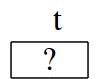
\includegraphics[scale=.5]{../img/java-tabl-repres2}\end{center}
  \item \java{t = new int[3];}
  \begin{center}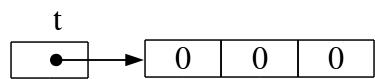
\includegraphics[scale=.5]{../img/java-tabl-repres1}\end{center}
 \end{itemize}
\end{frame}

\begin{frame}[fragile]{Repr�sentation}
  \emph{Exemple} : \java|int[][] t = new int[3][2];|
  \begin{itemize}
  \item Un tableau de 3 tableaux de 2 entiers
  \bigskip
  \begin{center}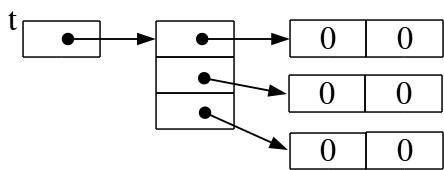
\includegraphics[scale=.4]{../img/java-tabl-dim2}\end{center}
  \item Repr�sentation interne $\not=$ vision classique
    \\
    \begin{small}
    \begin{center}\begin{tabular}{|c|c|}\hline ~ ~ 0 ~ ~ & ~ ~ 0 ~ ~ \\ \hline ~ ~ 0 ~ ~ & ~ ~ 0 ~ ~ \\ 
                                        \hline ~ ~ 0 ~ ~ & ~ ~ 0 ~ ~ \\ \hline\end{tabular}\end{center}
    \end{small}
 \end{itemize}
\end{frame}

\begin{frame}{Repr�sentation}
  Pour les tableaux � plusieurs dimensions
  \begin{itemize}
  \item Chaque �l�ment d'un tableau � deux dimensions est un tableau ind�pendant
  \item La taille ne fait pas partie du type
  \item $\Rightarrow$ Chaque �l�ment peut �tre d'une \emph{taille diff�rente}
  \end{itemize}
  \medskip
  \begin{center}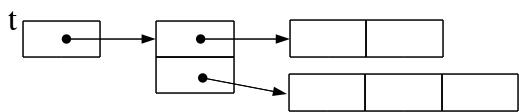
\includegraphics[scale=.5]{../img/java-tabl-dim2b}\end{center}
\end{frame}

\begin{frame}[fragile]{Cr�ation}
  On peut omettre les derni�res tailles
  \begin{itemize}
  \item Le tableau est cr�� en partie
  \item \emph{Exemple} :
  \begin{Java}
  int[][] t;
  t = new int[3][];
  \end{Java}
  \begin{center}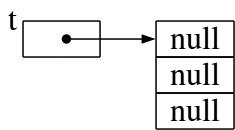
\includegraphics[scale=.5]{../img/java-tabl-new2}\end{center}
  \item Le reste sera cr�� plus tard
  \end{itemize}
\end{frame}

\begin{frame}[fragile]{Cr�ation}
  Cr�ation en donnant les valeurs
  \begin{grammaire}[fontsize=\footnotesize]
  \nterm{ArrayCreationExpression} :
   \term{new} \nterm{TypeName} \nterm{Dims} \nterm{ArrayInitializer}  

  \nterm{ArrayInitializer} :
     \term{\{} \nterm{VariableInitializers}\opt \term{,}\opt \term{\}}

  \nterm{VariableInitializers} :
     \nterm{VariableInitializer}
     \nterm{VariableInitializers} \term{,} \nterm{VariableInitializer}

  \nterm{VariableInitializer} :
     \nterm{Expression}
     \nterm{ArrayInitializer}
  \end{grammaire}
\end{frame}

\begin{frame}[fragile]{Cr�ation}
\emph{Exemple} de format long
  \begin{Java}
  int[] entiers = new int[] {4,5,6};
  int[] entiers;
  entiers = new int[] {4,5,6};
  \end{Java}
\medskip
�criture abr�g�e (uniquement � la d�claration)
  \begin{Java}
int[] entiers = {4,5,6}; // �criture abr�g�e accept�e
int[] entiers;
entiers = {4,5,6}; // Erreur � la compilation
  \end{Java}
\medskip
\emph{Exercice} : Donnez la repr�sentation m�moire
  \begin{itemize}
  \item \java|int[][] entierss = {{1,2},{3,4,5}};|
  \item \java|int[][] entierss = {{1,2},null};|
  \end{itemize}
\end{frame}

\begin{frame}[fragile]{Cr�ation}
  \emph{Exercice} : Les cr�ations suivantes sont-elles correctes ? Pourquoi ?
  \begin{itemize}
  \item \java|int[][] entierss = new int[2];|
  \item \java|int[][] entierss = new int[] {1,2};|
  \item \java|int[][] entierss = new int[] {{1},{2}};|
  \item \java|int[][] entierss = new int[3][2] {1,2};|
  \item \java|int[][] entierss = new int[3][2] {null,null};|
  \end{itemize}
\end{frame}

\begin{frame}[fragile]{Cr�ation}
\emph{Exercice} : Lecture d'un vecteur.
\\ Attention ! Ceci n'est pas correct. Pourquoi ?
\begin{Java}
  import java.util.Scanner;
  public class LectureVecteur {
     public static void main(String[] args) {
        Scanner clavier = new Scanner(System.in);
        int[] vecteur;    // le vecteur � lire
        int   taille;     // taille du vecteur
        taille = clavier.nextInt();
        for (int i=0; i<taille; i=i+1)
           vecteur[i] = clavier.nextInt();
     }
  }
\end{Java}
\end{frame}

\subsection{Taille}

\begin{frame}[fragile]{Taille}
La taille doit �tre un \java|int|
 \begin{itemize}
  \item Jusqu'� 2 milliards d'�l�ments ;-)
  \item Peut �tre \emph{nulle}
    \begin{itemize}
    \item ex : \java|int[][] entierss = new int[0][2];|
    \item peut avoir un sens comme cas limite
    \end{itemize}
  \item Ne peut \emph{pas} �tre \emph{n�gative}
    \begin{itemize}
    \item sinon une exception est lanc�e
    \item pas v�rifi� � la compilation m�me si constante
    \end{itemize}
  \item Est une expression g�n�rale
    \begin{itemize}
    \item ex : \java|int[] entiers = new int[clavier.nextInt()];|
    \end{itemize}
  \end{itemize}
\end{frame}

\begin{frame}[fragile]{Taille}
\emph{Rappel} : on connait la taille via \java|length|
\par\medskip Si plusieurs dimensions
    \begin{itemize}
    \item Taille (potentiellement) diff�rente d'une ligne � l'autre
    \item $\Rightarrow$ Sp�cifier la ligne
    \item Exemple :
      \begin{Java}
  int[][] entierss = {{1,2},{2,3,4}};
  System.out.println( "Nombre d'�l�ments = "
      + (entierss[0].length + entierss[1].length) );
      \end{Java}
    \end{itemize}
\end{frame}

\begin{frame}[fragile]{Taille}
\emph{Exemple} : Que va imprimer le code suivant?
\begin{Java}
  package be.heb.esi.lg1.tutorials.tableaux;

  public class ParcoursLigneParLigne{
     public static void main(String[] args){
        String[][] entierss = {{"00","01","02","03","04"},
                             {"10","11","12","13","14"}};
        for(int i = 0; i < entierss.length; i = i + 1)
           for(int j = 0; j < entierss.length; j = j + 1)
              System.out.println(entierss[i][j]);
     }
  }
\end{Java}
\end{frame}

\begin{frame}[fragile]{Taille}
\emph{Exemple} : Parcours d'un tableau d'entiers � deux dimensions ligne par ligne
\begin{Java}
  package be.heb.esi.lg1.tutorials.tableaux;

  public class ParcoursLigneParLigne{
     public static void main(String[] args){
        String[][] entierss = {{"00","01","02","03","04"},
                          {"10","11","12","13","14"}};
        for(int i = 0; i < entierss.length; i = i + 1)
           for(int j = 0; j < entierss[i].length; j = j + 1)
              System.out.println(entierss[i][j]);
     }
  }
\end{Java}
\end{frame}

\subsection{Parcours}

\begin{frame}[fragile]{foreach}
\emph{Rappel} : Le \emph{foreach} simplifie le parcours d'un vecteur
\begin{itemize}
\item[]
  \begin{Java}
  public static void afficher( int[] entiers )  {
    for( int val : entiers ) {
      System.out.print( val + " " );
    }
  }
  \end{Java}
\end{itemize}
\medskip
On peut l'utiliser pour une matrice
\begin{itemize}
\item version qui utilise le parcours d'un vecteur
\begin{Java}
  public static void afficher( int[][] mat )  {
    for( int[] ligne : mat ) {
      afficher( ligne );
      System.out.println();
    }
  }
\end{Java}
\end{itemize}
\end{frame}

\begin{frame}[fragile]{foreach}
\begin{itemize}
\item version qui refait tout
\begin{Java}
  public static void afficher( int[][] mat )  {
    for( int[] ligne : mat ) {
      for( int val : ligne ) {
        System.out.print( val + " " );
      }
      System.out.println();
    }
  }
\end{Java}
 \item Peut-on utiliser le \emph{foreach} pour un parcours \emph{colonne par colonne} ?
\end{itemize}
\end{frame}

\subsection{Assignation en bloc}

\begin{frame}[fragile]{Assignation}
  Un tableau est de type r�f�rence
  \begin{itemize}
  \item \emph{L'assignation} d'un tableau � un autre \emph{copie la r�f�rence} (et pas le tableau)
  \item Exemple : \java|int[] t1 = {4,5,6}, t2 = t1;|
  \medskip
  \begin{center}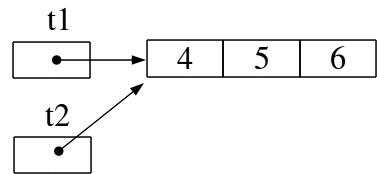
\includegraphics[scale=.5]{../img/java-tabl-ass1}\end{center}
  \end{itemize}
\end{frame}

\begin{frame}[fragile]{Assignation}
  \emph{Exemple} : \java|int[] t1 = {4,5,6}, t2 = {1,2}; t2 = t1;|
  \begin{center}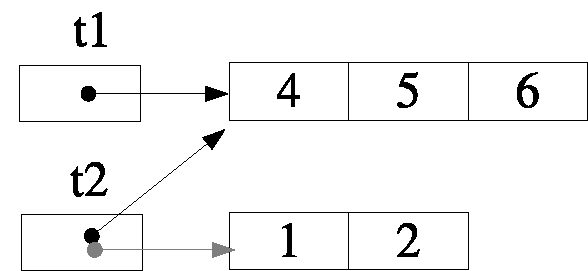
\includegraphics[scale=.7]{../img/java-tabl-ass2}\end{center}
  \begin{itemize}
  \item L'ancien tableau n'est plus r�f�renc�
  \item La place m�moire est r�cup�r�e (par le \textit{garbage collector})
  \end{itemize}
\end{frame}

\begin{frame}[fragile]{Acc�s aux �l�ments}
Pour acc�der � un �l�ment on donne tous les indices
      \\\emph{Exemple}
      \begin{Java}
  int[][][] t = new int[4][5][3];
  t[0][2][1] = 1; // Faites un sch�ma m�moire !
      \end{Java}
\bigskip
Cela a du sens de n'en sp�cifier que certains
      \\\emph{Exemple}
      \begin{Java}
  int[] t = { 4,5,6 };
  int[][] t2 = { {1,2,3}, {4,5} };
  t2[1] = t; // Faites un sch�ma m�moire !
      \end{Java}
\end{frame}

\begin{frame}[fragile]{Cr�ation}
\emph{Exemple} : Autre �criture pour la cr�ation d'un tableau.
\begin{Java}
  int[][] t = new int[3][2];
\end{Java}
Pourrait s'�crire
\begin{Java}
  int[][] t;
  t = new int[3][];
  for (int i=0; i<3; i=i+1)
     t[i] = new int[2];
\end{Java}
\end{frame}

\begin{frame}[fragile]{Cr�ation}
\emph{Exemple} : Cr�ation d'un tableau triangulaire
\begin{Java}
  package be.heb.esi.lg1.tutorials.tableaux;

  public class TableauTriangulaire{
     public static void main(String[] args){
        int[][] t;
        t = new int[3][];
        for (int i=0; i<3; i=i+1)
           t[i] = new int[i+1];
     }
  }
\end{Java}
\end{frame}

\begin{frame}[fragile]{Cr�ation}
\emph{Exemple} : Triangle de Pascal
\begin{Java}
  import java.util.Scanner;
  public class TrianglePascal {
     public static void main(String[] args) {
        Scanner clavier = new Scanner(System.in);
        int taille = clavier.nextInt();
        int[][] pascal; // le triangle de Pascal
        pascal = new int[taille][];
        for (int i=0; i<taille; i=i+1) {
           pascal[i] = new int[i+1];
           pascal[i][0] = 1;
           pascal[i][i] = 1;
           for(int j=1; j<i; j=j+1)
              pascal[i][j] = pascal[i-1][j-1]+pascal[i-1][j];
        }
     }
  }
\end{Java}
\end{frame}

\subsection{Erreurs et exceptions}

\begin{frame}[fragile]{Erreurs et exceptions}
Lors de l'acc�s � un �l�ment
\begin{itemize}
\item Si l'indice n'est pas valide (par rapport � la taille du tableau), 
la \sigle{JVM} lance une exception (\emph{ArrayIndexOutOfBoundException})
\item \emph{Exemple} :
\begin{Java}
  int[] entiers = {7,14,0};
  int i1 = entiers[-1]; // erreur � l'ex�cution
  int i2 = entiers[3]; // erreur � l'ex�cution
  int i3 = entiers[0.0]; // erreur � la compilation
\end{Java}
\end{itemize}
\end{frame}

\begin{frame}[fragile]{Erreurs et exceptions}
La \sigle{JVM} lance aussi une exception si le tableau est � \java|null| (\emph{NullPointerException})
\begin{itemize}
\item \emph{Exemple} :
\begin{Java}
  int[][] entierss = {{1,2},null};
  int[] entiers = entierss[1]; // OK
  int entier = entierss[1][0]; // erreur � l'ex�cution
\end{Java}
\end{itemize}
\end{frame}

\begin{frame}[fragile]{Erreurs et exceptions}
Lors d'une assignation
\begin{itemize}
\item Comme dans toute assignation, il faut que les \emph{types correspondent}
\item Exemple :
\begin{Java}
  int[] t1 = {4,5,6};
  boolean[] t2 = t1; // erreur � la compilation
\end{Java}
\item \emph{Exemple} :
\begin{Java}
  int[][] t1 = {{4,5,6},{1,2}};
  int[] t2 = t1[0]; // t2={4,5,6};
\end{Java}
\end{itemize}
\end{frame}

\subsection{Tableau et m�thode}

\begin{frame}[fragile]{M�thode}
Passer un tableau en param�tre
\\= Passer une copie de la r�f�rence au tableau
\begin{itemize}
\item La m�thode agit sur le tableau et pas une copie
\end{itemize}
\medskip
\emph{Exemple} : Un tableau en argument
\begin{itemize}
\item[]
\begin{Java}
  public class TableauEnArgument {
     public static void iniTableau(int[] tab) {
        for(int i=0; i<tab.length; i++)
           tab[i]=0;
     }

     public static void afficheTab(int[] tab) {
        for(int i=0; i<tab.length; i++)
           System.out.print(tab[i]+" ");
     }
  }
\end{Java}
\end{itemize}
\end{frame}

\begin{frame}[fragile]{M�thode}
\emph{Exemple} : Utilisation
\begin{itemize}
\item[]
\begin{Java}
  public class Test {
     public static void main(String[] args) {
        int[] tableau = new int[]{8,4,3,9};
        System.out.print("tableau avant: ");
        TableauEnArgument.afficheTab(tableau);
        TableauEnArgument.iniTableau(tableau);
        System.out.print("\ntableau apr�s: ");
        TableauEnArgument.afficheTab(tableau);
    }
  }
\end{Java}
\end{itemize}
\end{frame}

\begin{frame}[fragile]{M�thode}
\emph{Exemple} : Un tableau en retour
\begin{itemize}
\item[]
\begin{Java}
  public static int[] tableauEnRetour(int n) {
     int[] tableau = new int[n];
     for(int i=0;i<n;i++)
        tableau[i]=i+1;
     return tableau;
  }
\end{Java}
\item Un appel de la m�thode \emph{tableauEnRetour} fournira une r�f�rence � un tableau
\item Il est possible de modifier les valeurs des �l�ments
\end{itemize}
\end{frame}

\begin{frame}[fragile]{M�thode principale}
La m�thode \java|main| re�oit un tableau en argument
\begin{Java}
  public static void main(String[] args)
\end{Java}
\begin{itemize}
\item Il s'agit d'\emph{arguments} fournis au programme
\item \emph{Comment ?} via la ligne de commande
\begin{Java}
  java Test mes arguments
\end{Java}
\item Arguments s�par�s par un (des) espace(s)
\end{itemize}
\end{frame}

\begin{frame}[fragile]{M�thode principale}
\emph{Exemple} :
\begin{Java}
  public class Miroir {
    public static void main(String[] args) {
      System.out.print(args.length + ": ");
      for(int i=args.length-1; i>=0; i--)
        System.out.print(args[i] + " ");
    }
  }
\end{Java}
\begin{Code}
  > java Miroir Un message � l'envers
  4: l'envers � message Un 
\end{Code} 
\begin{Java}
  > java Miroir "Un message � l'envers"
  1: Un message � l'envers 
\end{Java} 
\end{frame}

\begin{frame}{Arrays}
La classe \emph{Arrays} offre des outils pratiques
\begin{itemize}
\item \emph{equals} : teste l'�galit� de tableaux
\item \emph{fill} : remplit tout un tableau avec une m�me valeur
\item \emph{toString} : retourne une chaine reprenant les �l�ments du tableau
\item \emph{copyOf}, \emph{sort}, \dots
\end{itemize}
\end{frame}



% ===== Cr�dits =====
\section*{Annexe}
\begin{frame}{Cr�dits}
Ce document a �t� produit avec les outils suivants
\begin{itemize}
\item {\small Les distributions \sigle{\emph{Ubuntu}} et/ou \sigle{\emph{debian}} 
du syst�me d'exploitation \sigle{\emph{Linux}}}
\item {\small \sigle{\emph{LaTeX}}/\sigle{\emph{Beamer}} comme syst�me d'�dition}
\item {\small \sigle{\emph{Git}} et \sigle{\emph{GitHub}} pour la gestion des versions et le suivi des corrections}
\item {\small Les outils \sigle{\emph{make}}, \sigle{\emph{rubber}}, \sigle{\emph{pdfnup}}, \dots}
\end{itemize}
\medskip
\href{http://creativecommons.org/licenses/by-sa/2.0/be}
{
\includegraphics[width=16mm]{../img/cc-by-nc-sa-80x15.png}}
\end{frame}

\end{document} 
 
